%---- Sample WMSU BSMATH BEAMER template ------
%---- Begin editing after PREAMBLE END at line 77------
%---- Created by: Christle Jude L. Maquilan - April 2022 --
%---- @jmaq03.jm@gmail.com -----

\documentclass[xcolor=dvipsnames,envcountsect]{beamer}

%------------------------------------------------
%------------------------------------------------
%------------------------------------------------
%------------------------------------------------
%------------------------------------------------
%----------▼▼▼▼▼ START PREAMBLE ▼▼▼▼▼----------

%-------- theme --------
\usetheme{Madrid}

%-------- color --------
\definecolor{crimsonred}{RGB}{153,0,0} % Official RGB code for Crimson Red
\usecolortheme[named=crimsonred]{structure}
%-------- set color of 'example block' to crimson theme --------
\setbeamercolor{block body example}{bg=white}
\setbeamercolor{block title example}{fg=white, bg=blue!50!black}

%-------- font --------
\setbeamerfont{structure}{family=\rmfamily,series=\bfseries}
\usefonttheme[stillsansseriftext]{structurebold}
\setbeamerfont{section in head/foot}{size=\tiny}

%-------- misc structure --------
\useoutertheme[footline=authortitle,subsection=false]{miniframes}
\useinnertheme{rounded}
\addtobeamertemplate{block begin}{}{\justifying}
\newtheorem{remark}[theorem]{Remark}
\renewcommand{\indent}{\hspace*{2em}}
\setbeamertemplate{theorems}[numbered]
\setbeamertemplate{caption}[numbered]
\usepackage[justification=centering]{caption}
\renewcommand{\qedsymbol}{$\blacksquare$}

%-------- packages to be used -------
\usepackage{amsmath,amsfonts,amssymb,amscd,amsthm}
\usepackage{graphicx,xcolor,comment}
\usepackage{mathrsfs} 
\usepackage{multirow}
\usepackage{array}
\usepackage{hyperref}
\usepackage{multicol}
\usepackage{ragged2e}
\usepackage{caption}
\usepackage[english]{babel}
\usepackage{rotating}
\usepackage{enumerate}
\usepackage{tikz}
\usepackage{bm}
\usepackage{csquotes}

%-------- for bibliography -----------------
\usepackage{biblatex}
\setbeamertemplate{bibliography item}{\insertbiblabel}
\addbibresource{References.bib}
\setbeamertemplate{frametitle continuation}{\frametitle{\color{white}List of References}}

%----------▲▲▲▲▲ PREAMBLE END ▲▲▲▲▲----------
%------------------------------------------------
%------------------------------------------------
%------------------------------------------------
%------------------------------------------------
%------------------------------------------------


%---------START EDITING HERE---------------------
\title[Quantitative Spectrum Analysis with MINS]{Quantitative Spectrum Analysis using Simulated Neutron Scattering Data}

\author [Cortes, J.A.]{\textbf{Jose Andres Cortes}}

\institute[The University of Texas at Arlington] {\emph{Adviser: }\textbf{Dr. Andrzej Korzeniowski}\\[1em]
Collaborators: Dr. Galina Yakubova, Dr. Aleksandr Kavetskiy, Dr. Allen Tobert\\[1em]
USDA Internship Project - MINS Simulation and Spectrum Deconvolution\\[1em]

\includegraphics[scale=0.3]{./Figures/WMSU CSM DMS.png}}

\date[April 2025]{\footnotesize Diagnostic Presentation - \textbf{April 2025}}

\begin{document}

\begin{frame}{\titlepage}\end{frame}

\begin{frame}{\frametitle{Presentation Outline}\tableofcontents}\end{frame}

%--------- BACKGROUND ----------------------
\section{Background}
\begin{frame}
  \frametitle{Application}
  \begin{itemize}
    \item Soil carbon: important for agriculture and emissions
    \item Lab method: Dry Combustion (accurate, expensive)
    \item MINS: on-site, non-destructive scanning system
    \item MINS: Mobile Inelastic Neutron Scattering System
    \item Role: simulate and analyze MINS neutron data
  \end{itemize}

    \begin{figure}
        \centering
        \begin{minipage}[b]{0.3\linewidth}
            \centering
            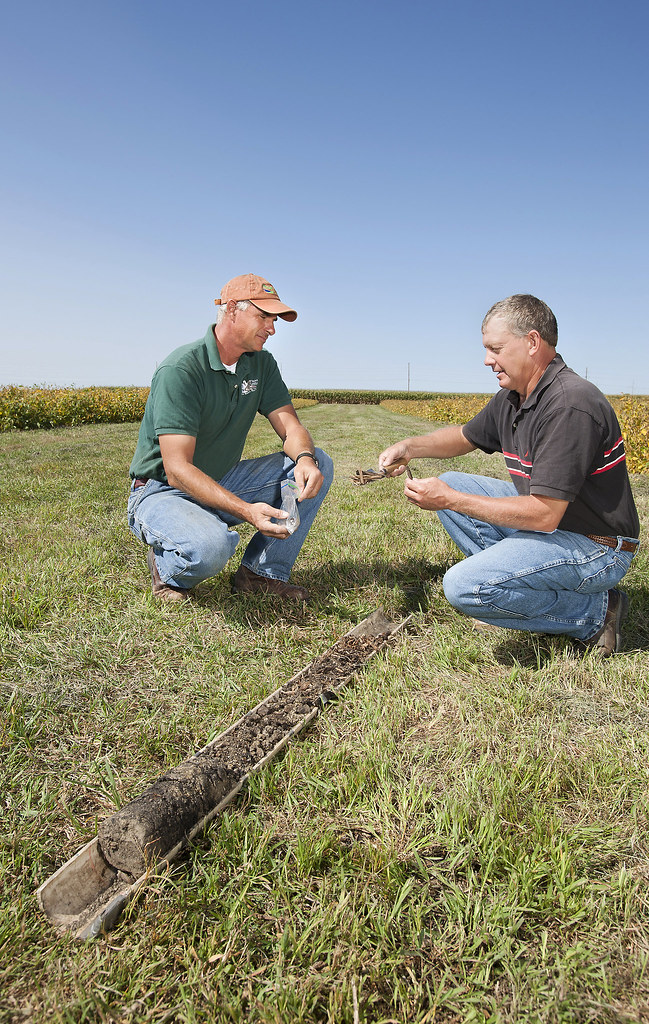
\includegraphics[clip, trim={0 0 0 4\linewidth}, width=\linewidth]{Figures/soil_core.jpg}
            \caption{Soil Core}
        \end{minipage}
        \begin{minipage}[b]{0.3\linewidth}
            \centering
            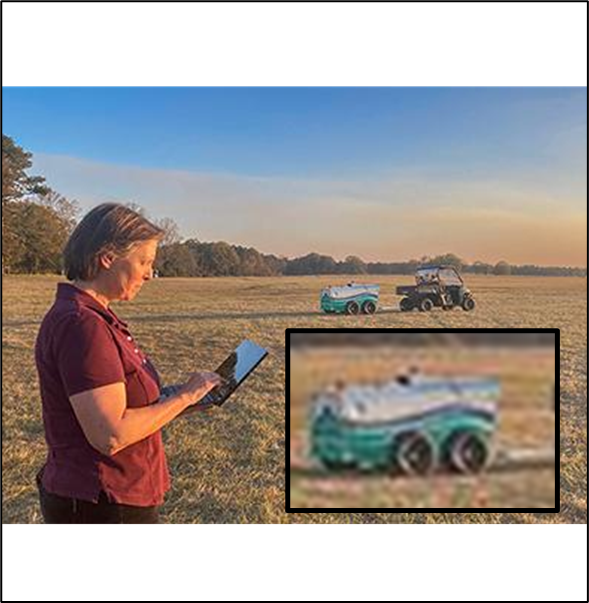
\includegraphics[width=\linewidth]{Figures/MINSInField.png}
            \caption{MINS}
        \end{minipage}
        % \caption{Soil Core and MINS}
        \label{fig:comparison}
    \end{figure}
\end{frame}

\begin{frame}
  \frametitle{Inelastic Neutron Scattering}
  \begin{itemize}
    \item Neutrons excite nuclei $\rightarrow$ emit gamma rays
    \item Signature peak: Carbon at 4.44 MeV (from 14 MeV neutron)
    \item Gamma peaks identify elements in soil
  \end{itemize}
  \begin{figure}
      \centering
      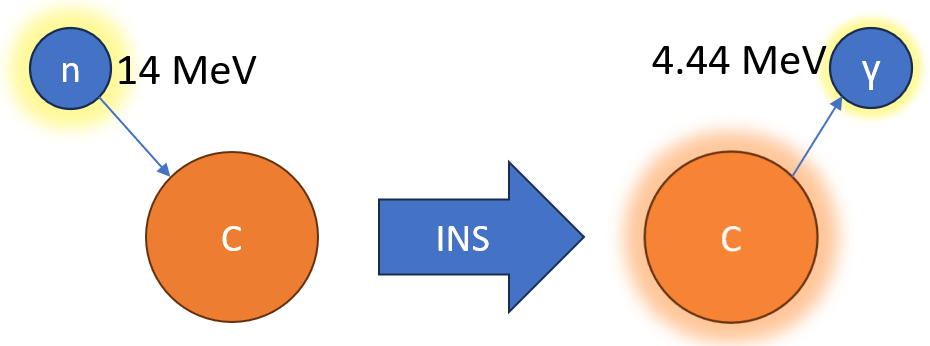
\includegraphics[width=\linewidth]{Figures/INS.png}
      % 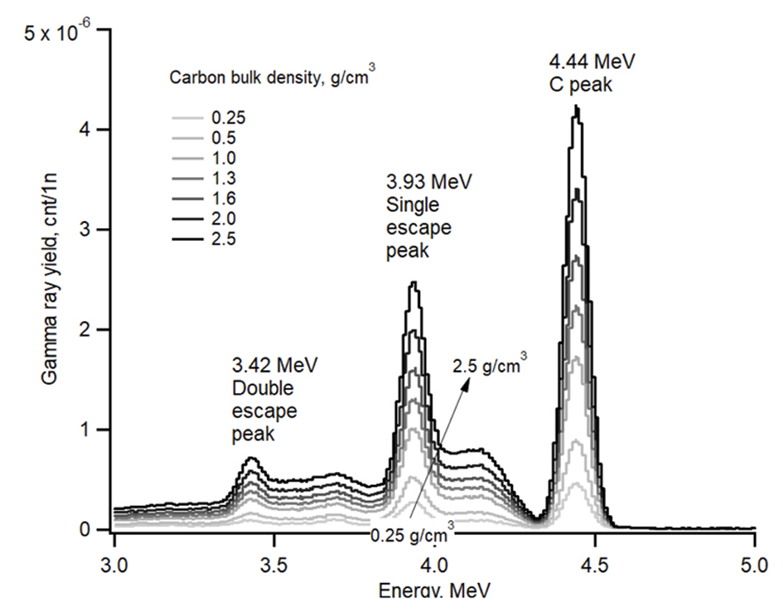
\includegraphics[width=0.5\linewidth]{Figures/inscrosssection.png}
      \caption{Inelastic Neutron Scattering on Carbon Atom}
      \label{fig:InelasticNeutronScattering}
  \end{figure}
\end{frame}

\begin{frame}
  \frametitle{Carbon Gamma Ray Cross Section}
  \begin{figure}
      \centering
      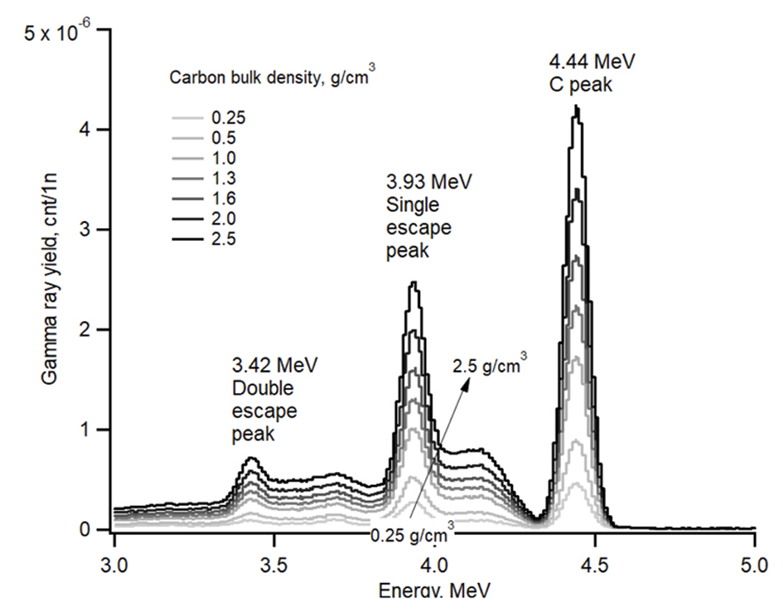
\includegraphics[width=.5\linewidth]{Figures/inscrosssection.png}
      \caption{Inelastic Neutron Scattering Cross Section on Carbon Atom}
      \label{fig:InelasticNeutronScatteringCS}
  \end{figure}
\end{frame}

\begin{frame}
  \frametitle{Simulating MINS - 1}
  \begin{itemize}
    \item Software: MCNP6.2 (Monte Carlo neutron transport)
    \item Geometry + material setup for full system
  \end{itemize}
  \begin{figure}
      \centering
      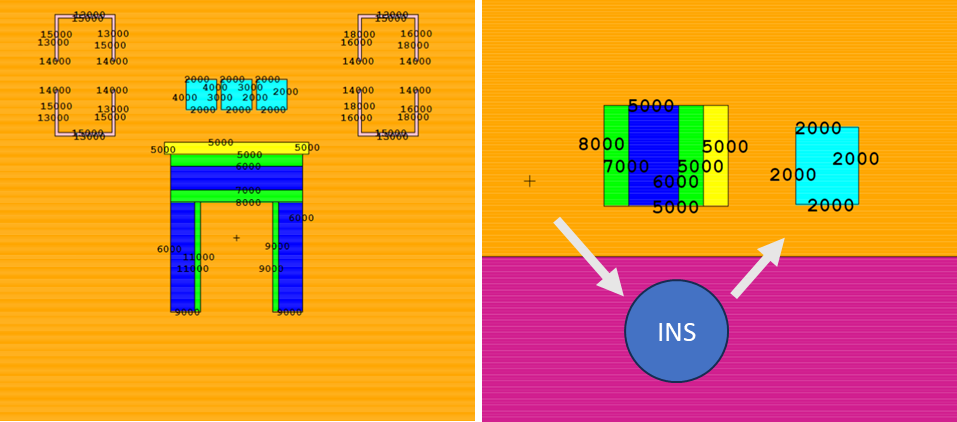
\includegraphics[width=\linewidth]{Figures/INSinMINS.png}
      \caption{Inelastic Neutron Scattering in MCNP}
      \label{fig:InelasticNeutronScatteringinMCNP}
  \end{figure}
\end{frame}

\begin{frame}
  \frametitle{Simulating MINS - 2}
  \begin{itemize}
    \item Fast neutrons interact with soil
    \item Emitted gamma rays detected and stored
  \end{itemize}
  \begin{figure}
      \centering
      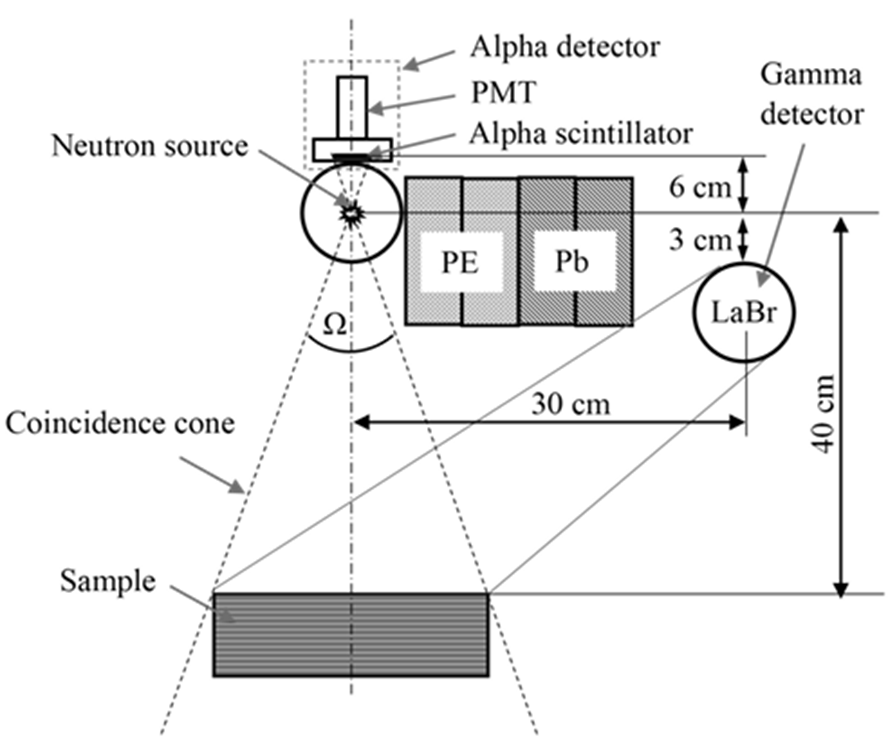
\includegraphics[width=.5\linewidth]{Figures/minsarchitecture.png}
      \caption{MINS Architecture}
      \label{fig:MINSArchitecture}
  \end{figure}
\end{frame}

\begin{frame}
  \frametitle{Defining Spectrums}
  \begin{itemize}
    \item Spectrum: histogram of energy counts
    \item One "history" = 50 ns neutron event window
    \item Use 10\textsuperscript{9} histories for high resolution
    \item Normalized spectrum = probability density
  \end{itemize}
  \begin{figure}
      \centering
      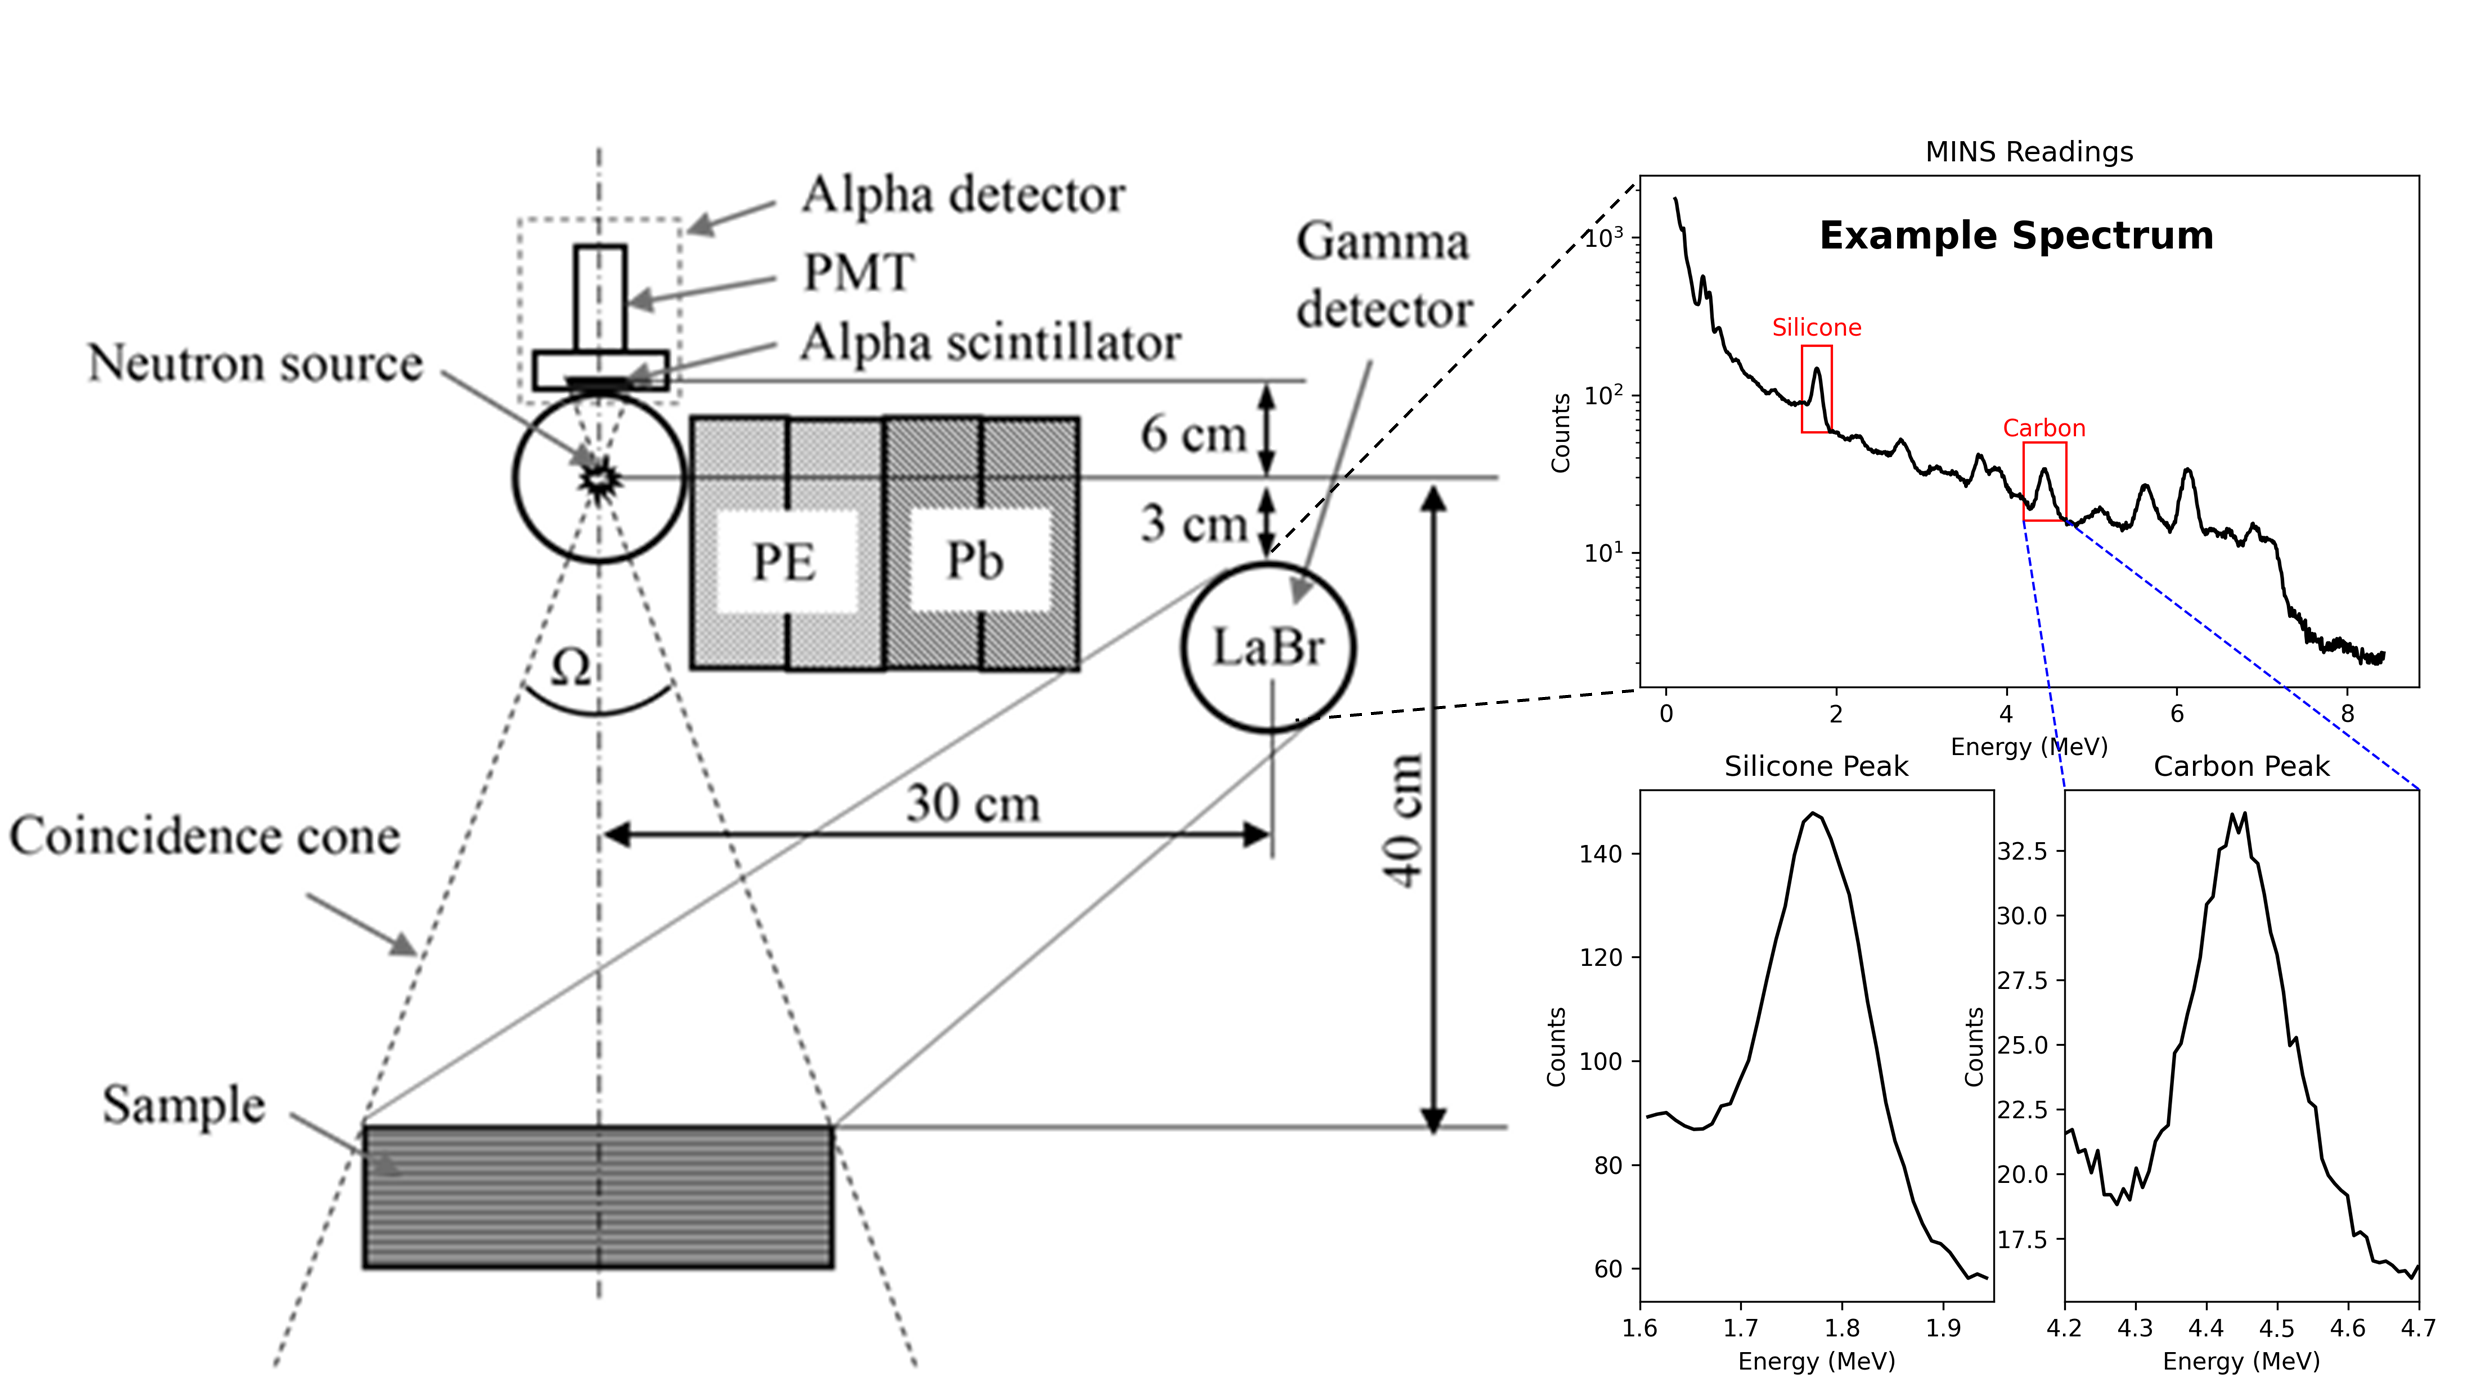
\includegraphics[width=.7\linewidth]{Figures/archtospec.png}
      \caption{Architecture to Spectrum}
      \label{fig:archtospec}
  \end{figure}
\end{frame}

\begin{frame}
  \frametitle{Spectrum Analysis}
  \begin{itemize}
    \item Peaks correspond to element emissions
    \item Goal: Deconvolve mix to get composition
  \end{itemize}
  \begin{figure}
      \centering
      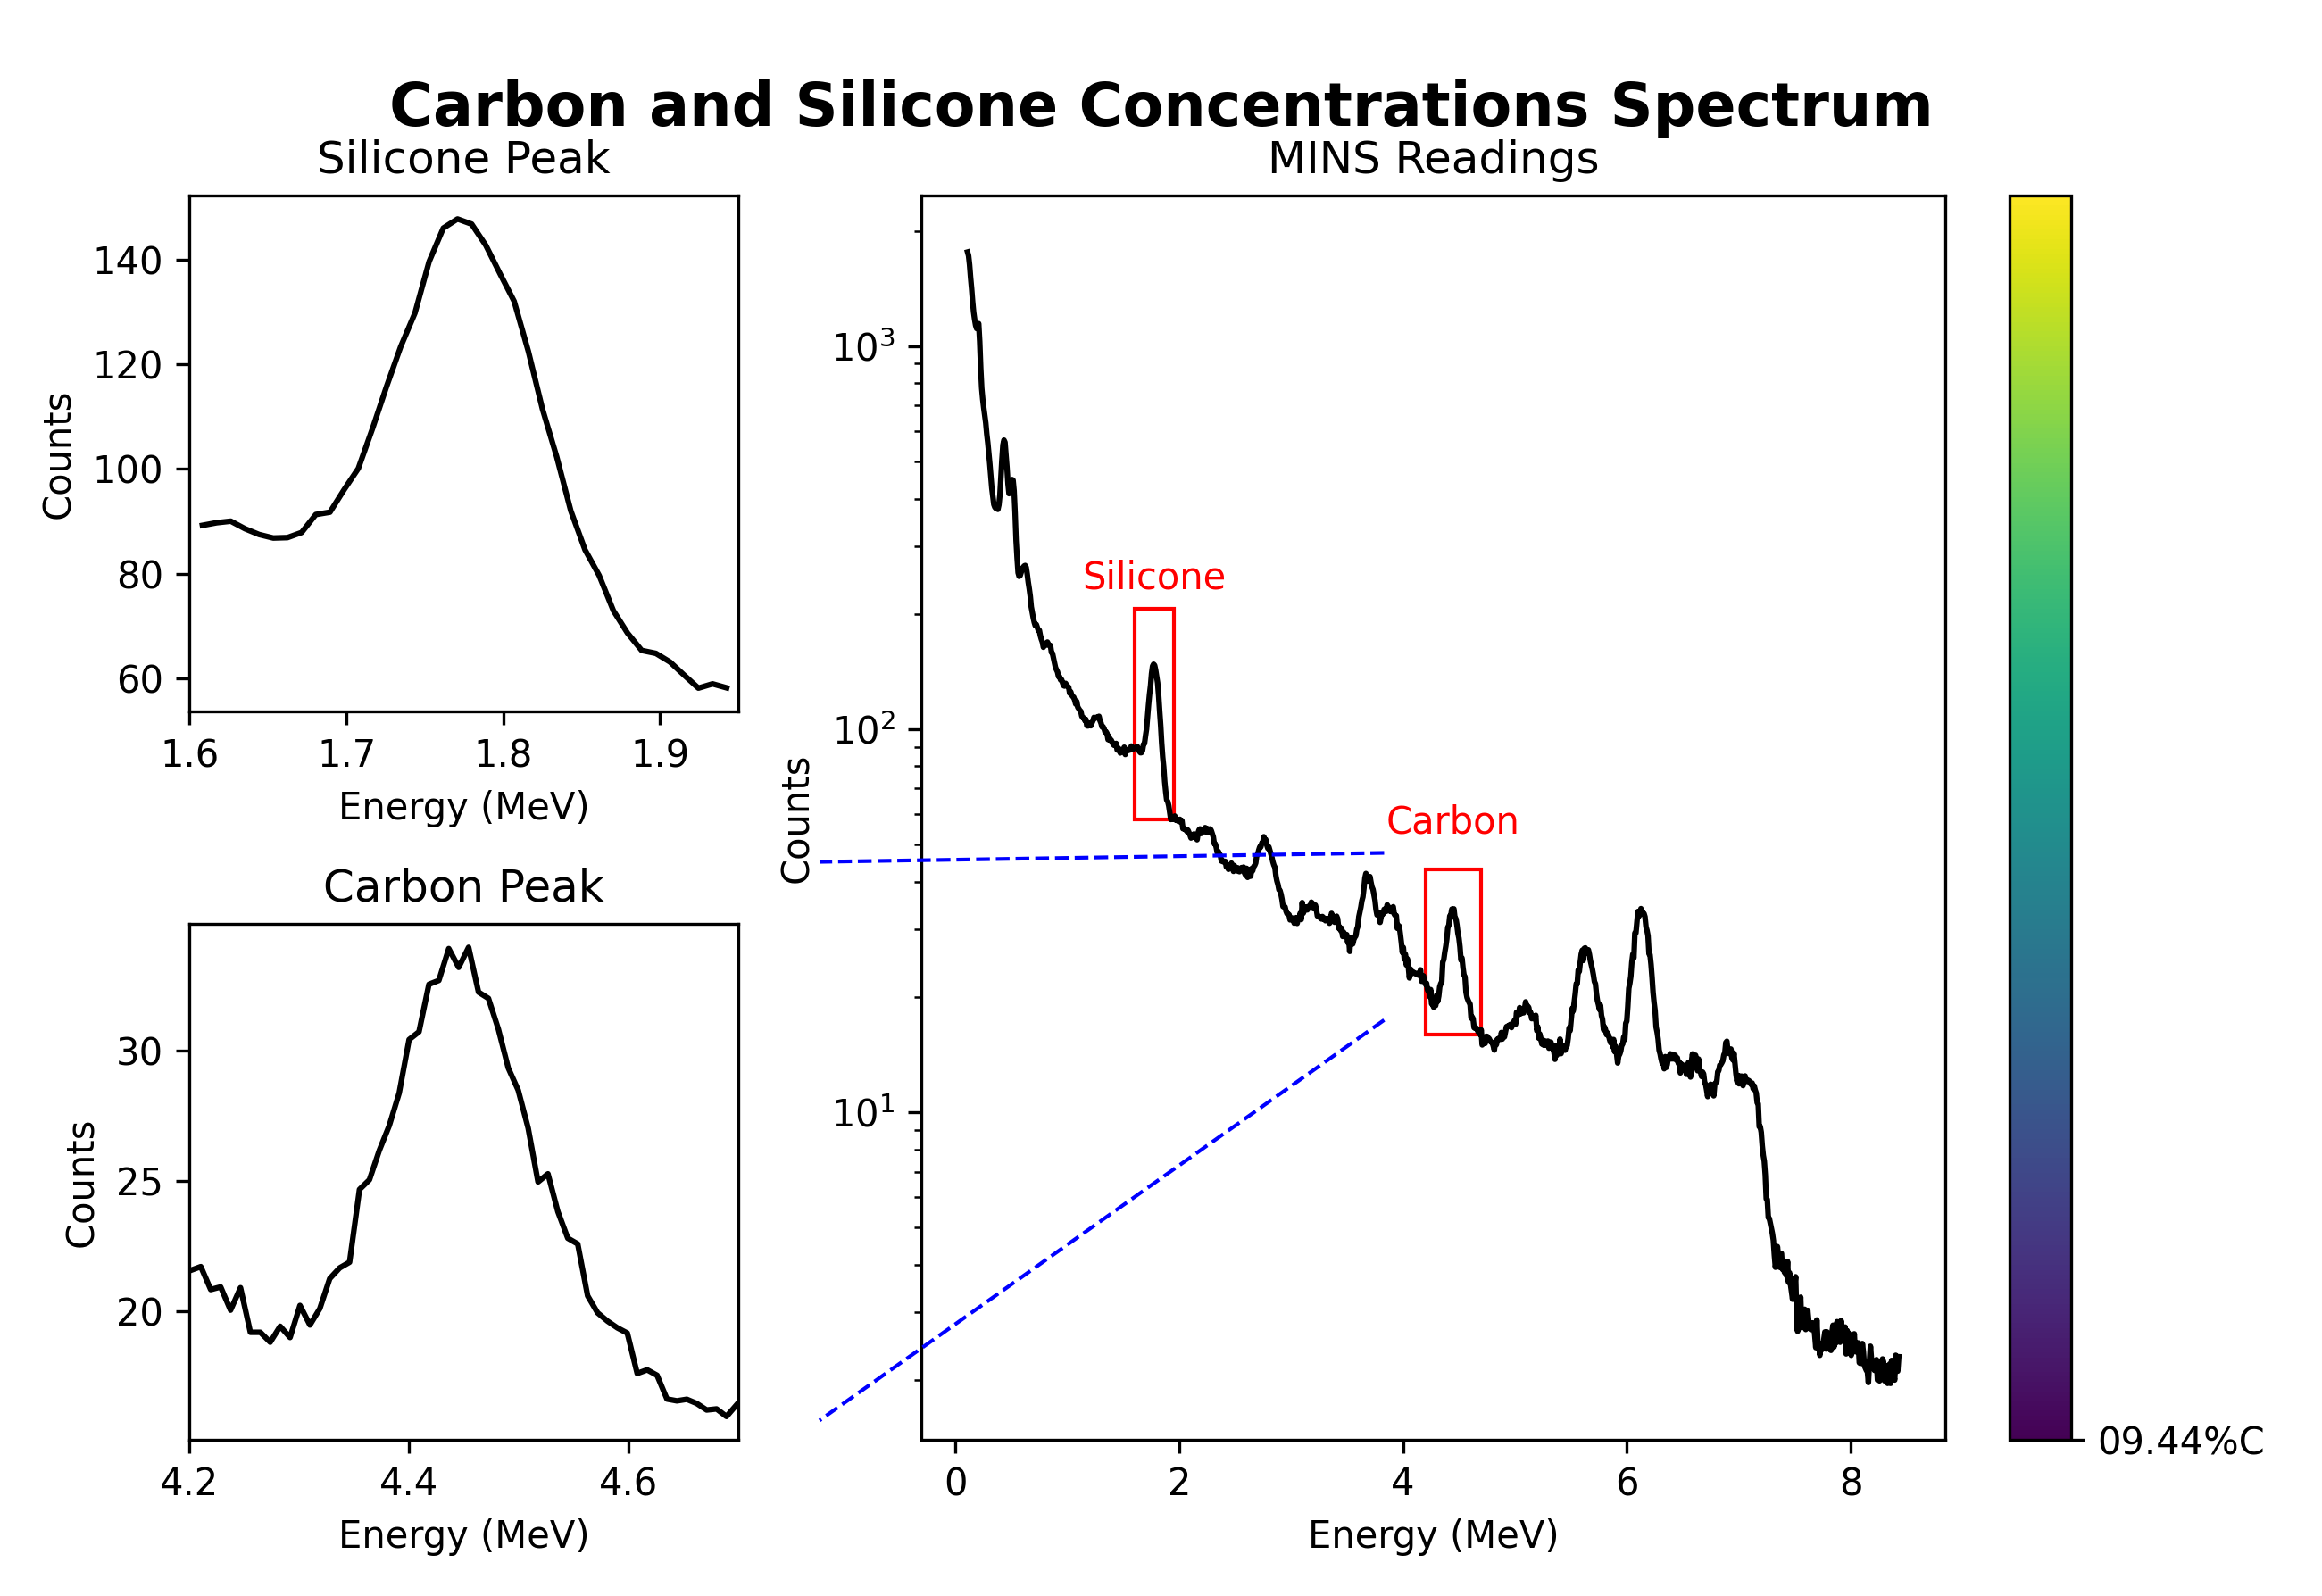
\includegraphics[width=.5\linewidth]{Figures/ExampleSpectrum.png}
      \caption{Example Spectrum}
      \label{fig:ExampleSpectrum}
  \end{figure}
\end{frame}

\begin{frame}
  \frametitle{Data Generation}
  \begin{itemize}
    \item Simulate samples: 0--30\% carbon + silicon base
    \item 10\textsuperscript{9} histories per sample
  \end{itemize}
  % carbon_silicone_concentrations.png
  \begin{figure}
      \centering
      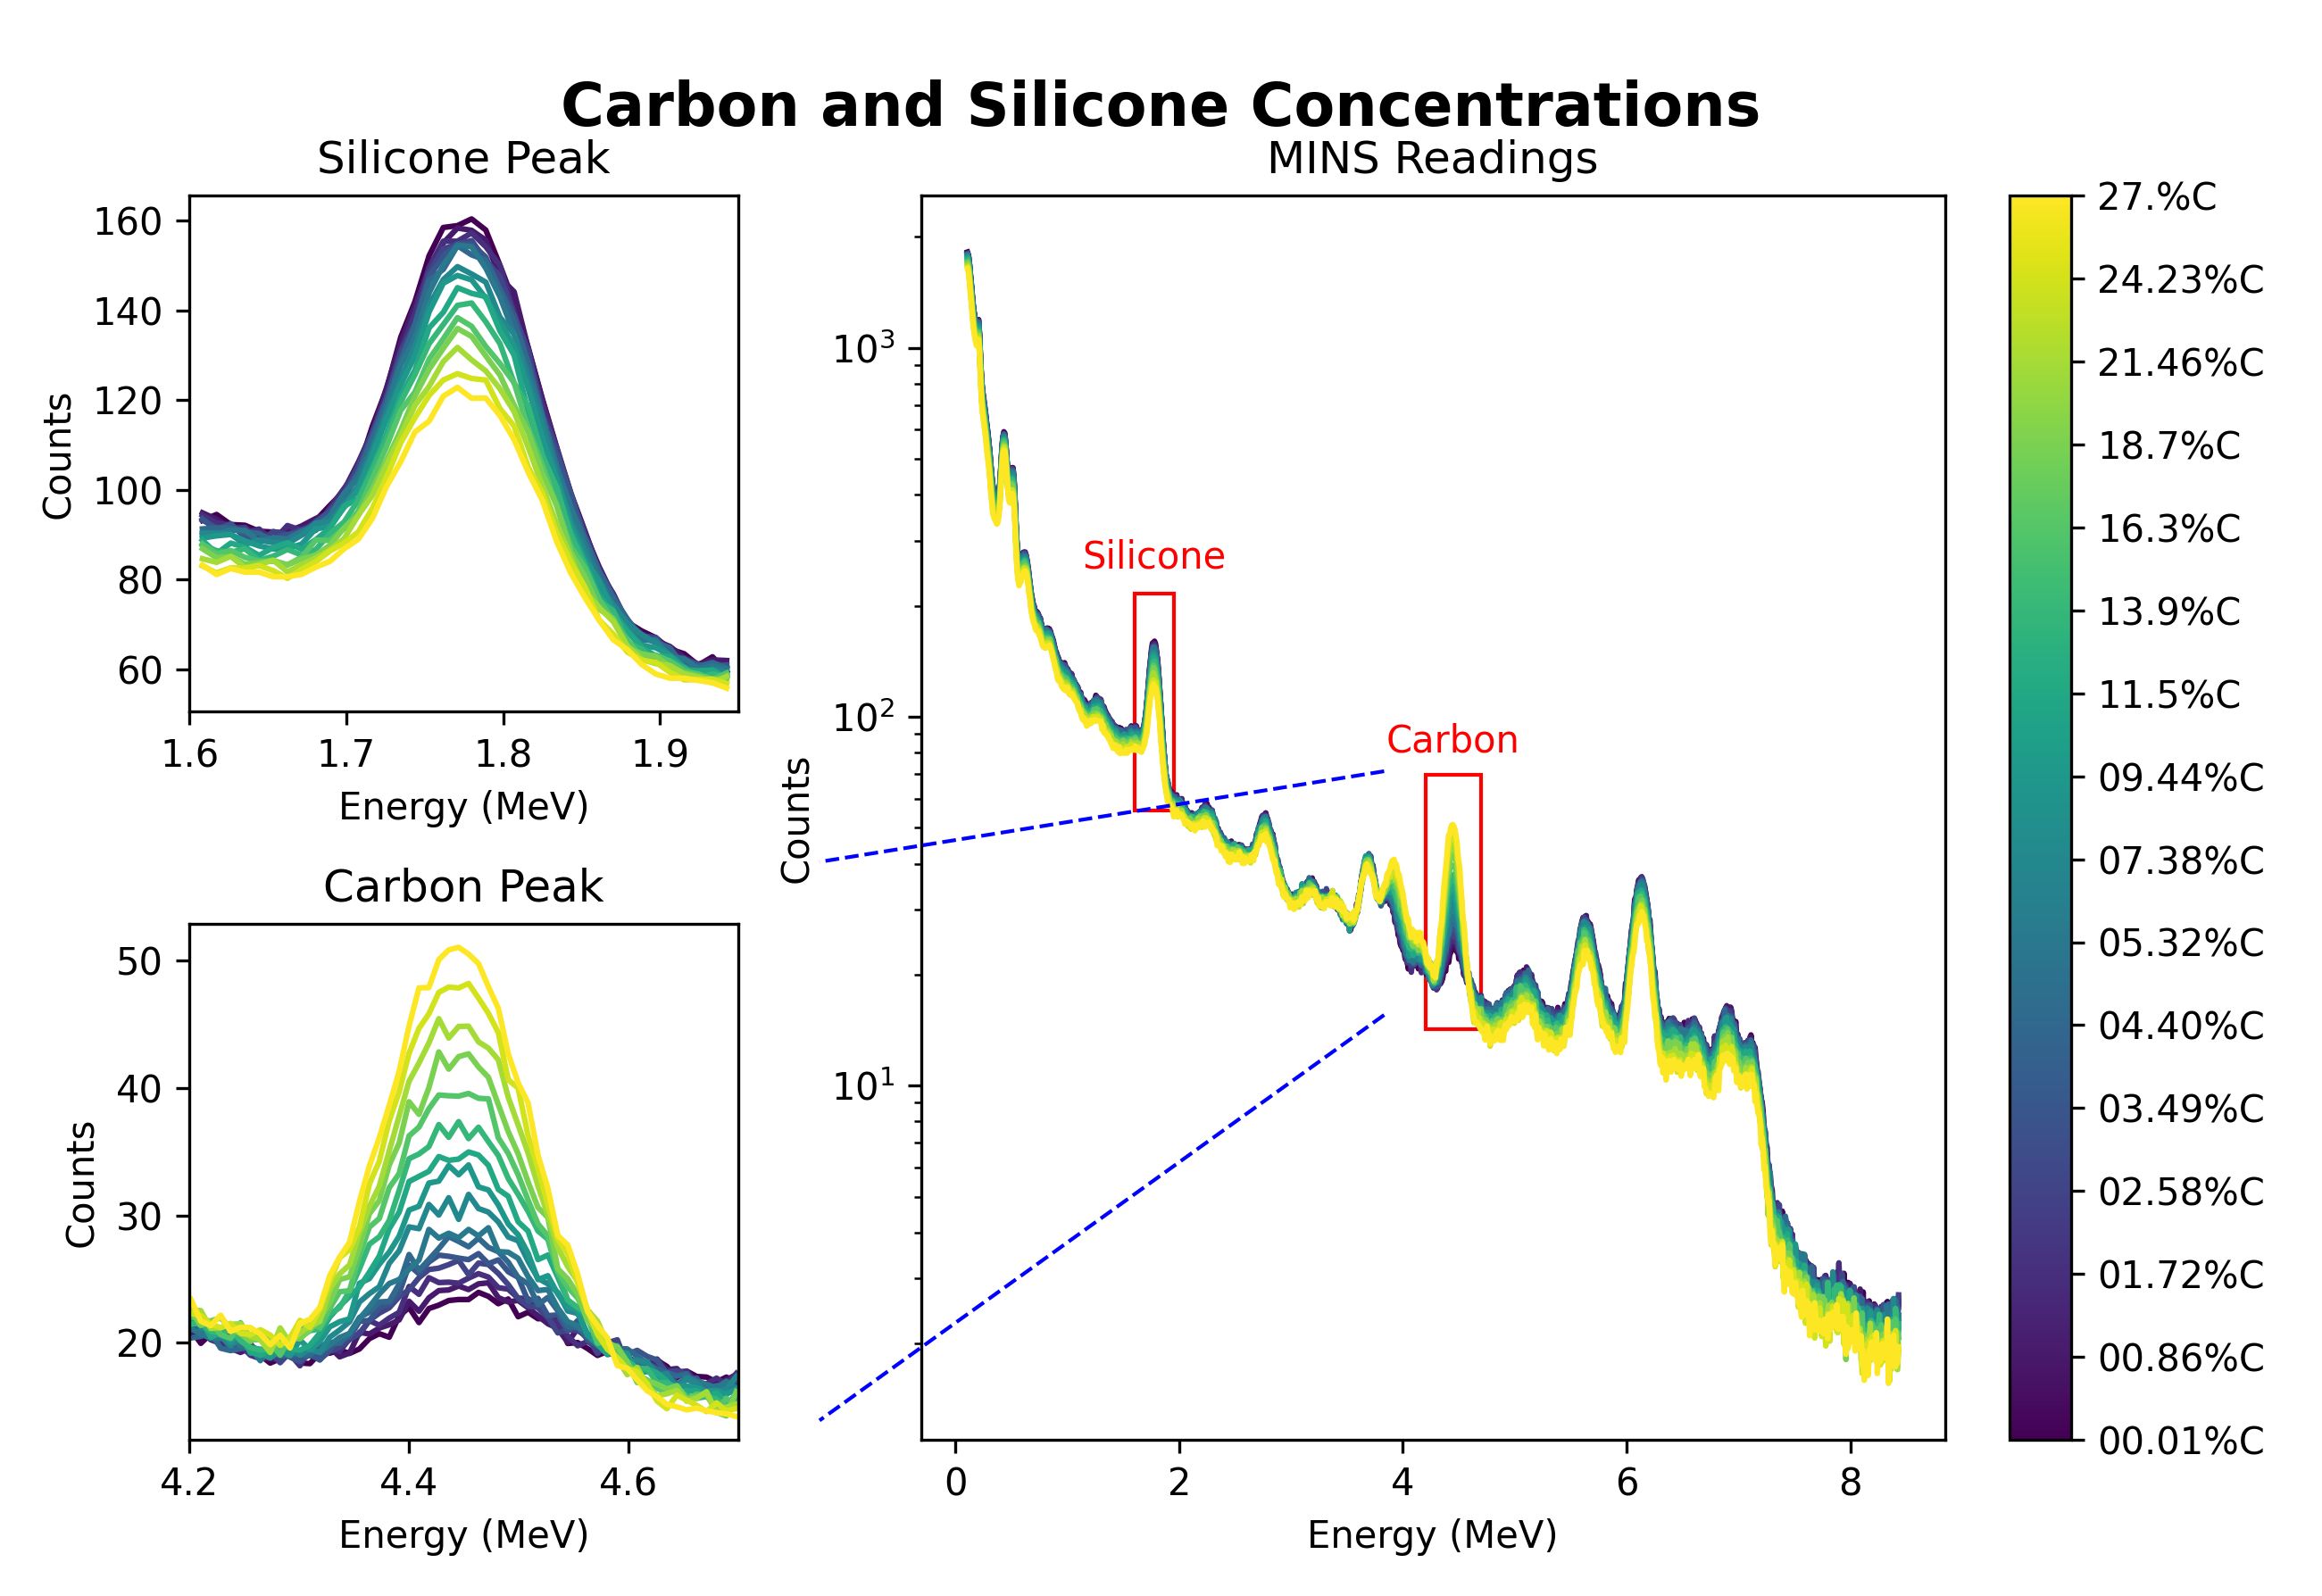
\includegraphics[width=.5\linewidth]{Figures/carbon_silicone_concentrations.png}
      \caption{Carbon and Silicon Concentrations}
      \label{fig:carbon_silicone_concentrations}
  \end{figure}
\end{frame}

%--------- ANALYSIS METHODS ----------------------
\section{Analysis Methods}
\begin{frame}
  \frametitle{Analysis Methods}
  \begin{itemize}
    \item Five methods: from classical to advanced
    \item Focus: identify carbon peak + baseline
  \end{itemize}
\end{frame}

\begin{frame}
  \frametitle{Classical Methods}
  \begin{itemize}
    \item Perpendicular Drop (PD): flat baseline from minimum
    \item Tangent Skim (TS): tangent line across valley
    \item Field data is noisy $\rightarrow$ limitations arise
  \end{itemize}
  \begin{figure}
      \centering
      \begin{minipage}[b]{0.3\linewidth}
          \centering
          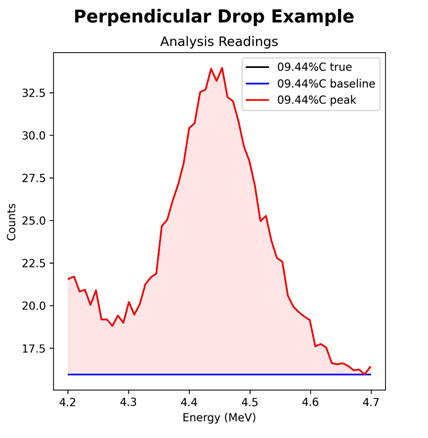
\includegraphics[width=\linewidth]{Figures/perpdropexample.png}
          \caption{PD Example}
          \label{fig:perpendiculardropexample}
      \end{minipage}
      % \hfill
      \begin{minipage}[b]{0.3\linewidth}
          \centering
          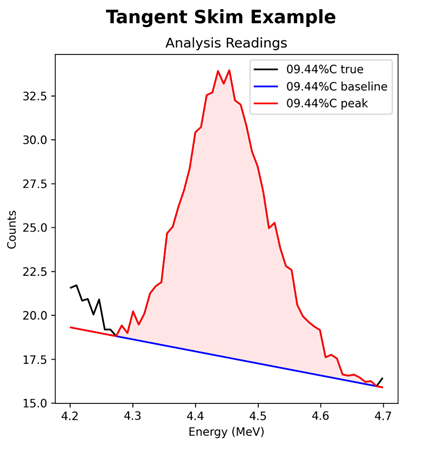
\includegraphics[width=\linewidth]{Figures/tangentskimexample.png}
          \caption{TS Example}
          \label{fig:tangentskimexample}
      \end{minipage}
  \end{figure}
\end{frame}

\begin{frame}
  \frametitle{Peak Fitting - Linear Baseline}
  \begin{itemize}
    \item Gaussian peak + linear baseline
    \item Fit using Levenberg-Marquardt algorithm
  \end{itemize}
  \begin{block}{Peak and Baseline Function}
    \begin{equation}
      f_{peak}(x) = A e^{-\frac{(x - B)^2}{2C^2}}
    \end{equation}
    \begin{equation}
      f_{baseline}(x) = mx + b
    \end{equation}
  \end{block}
  % Carbon Peak Fit Linear Baseline Example.png
  \begin{figure}
      \centering
      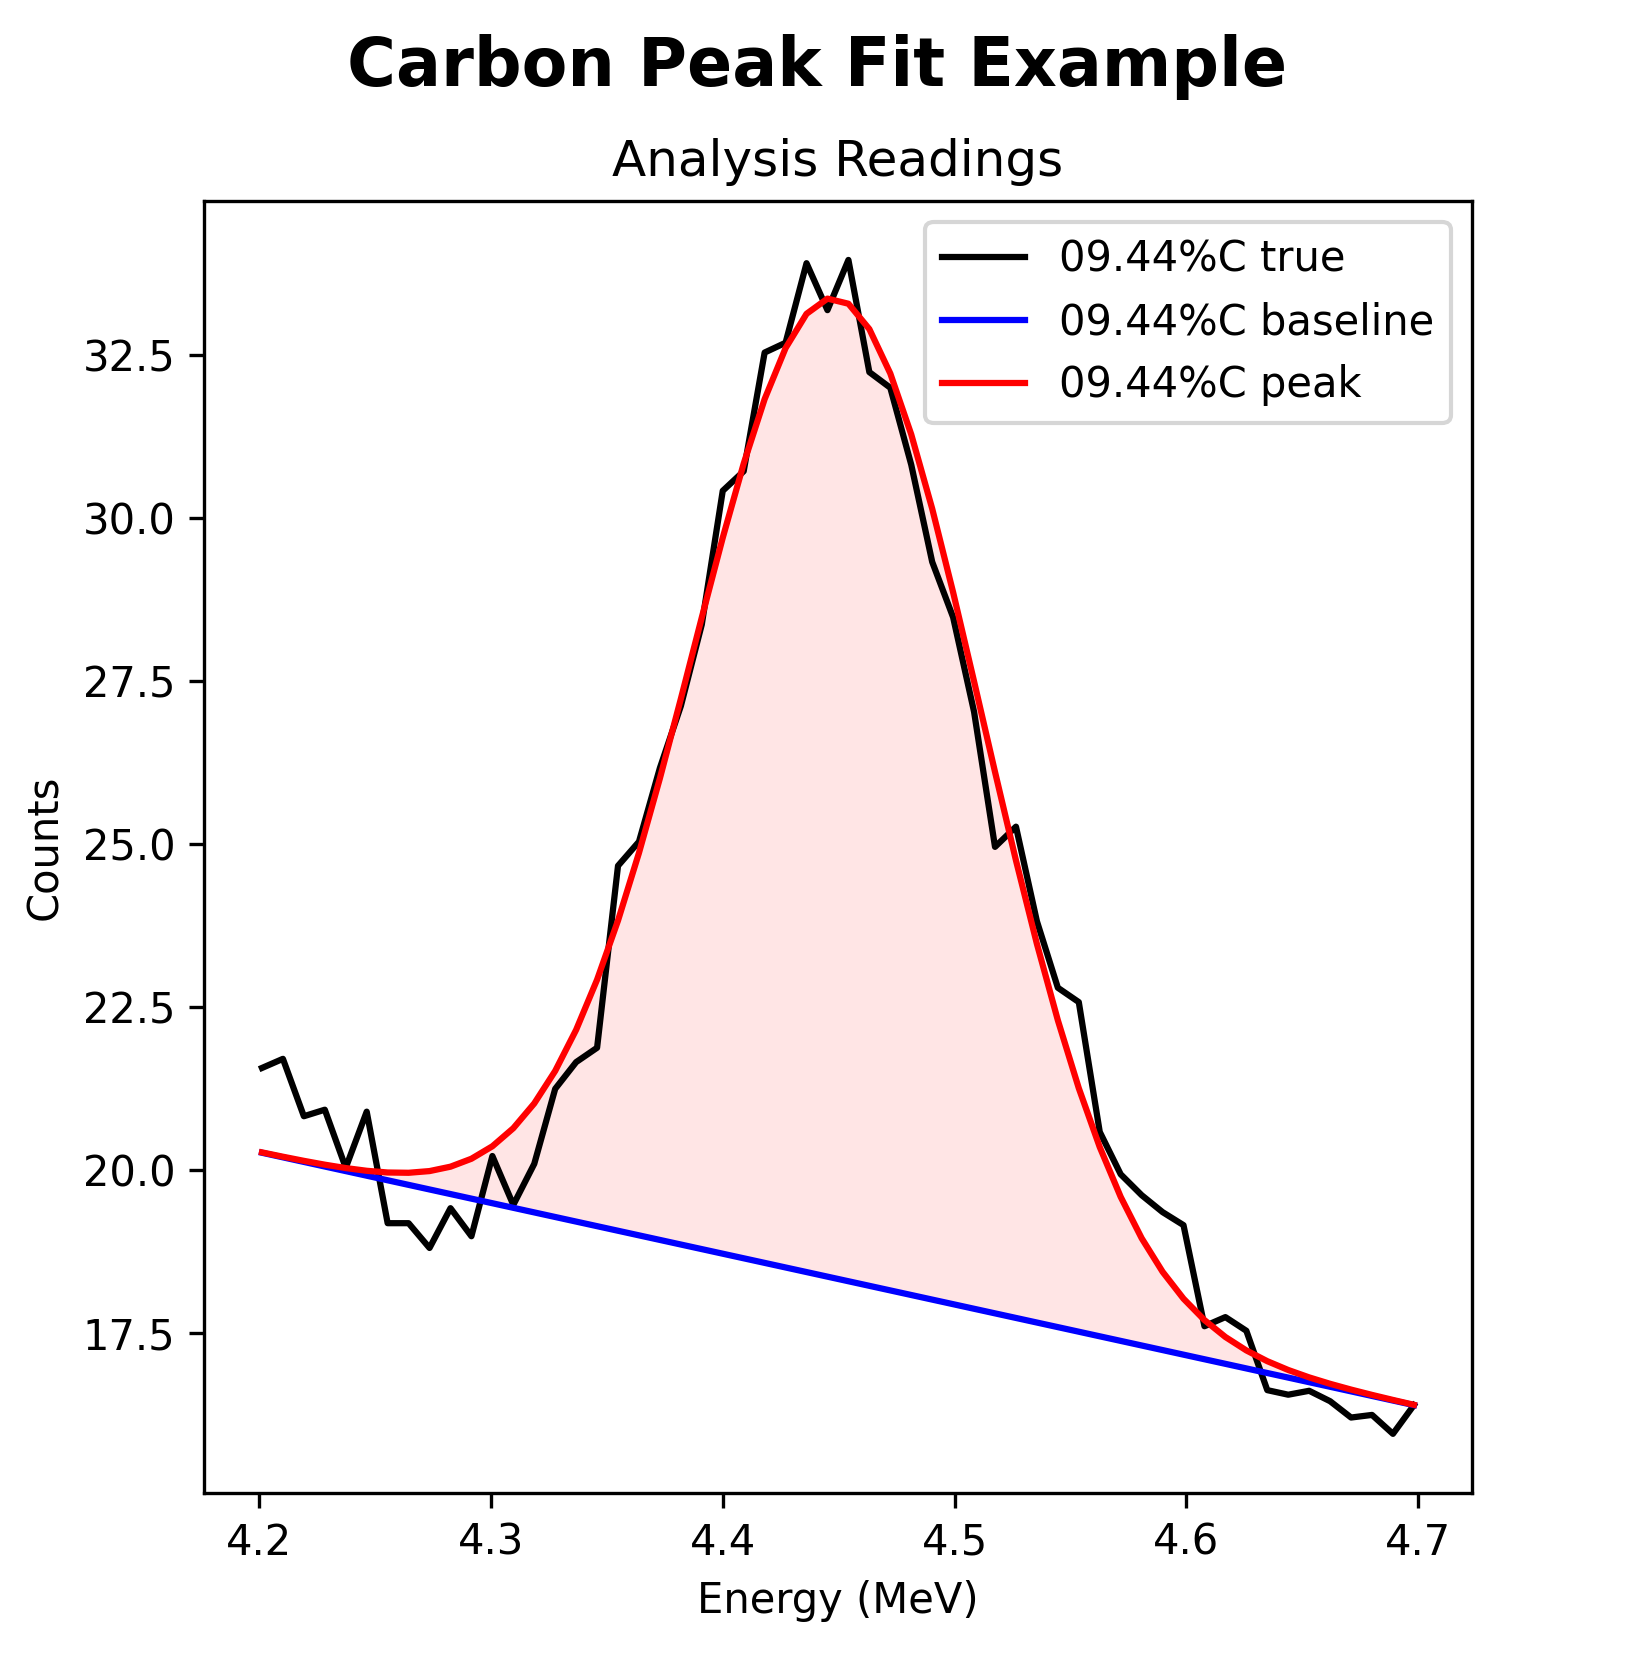
\includegraphics[width=.2\linewidth]{Figures/CarbonPeakFitLinearBaselineExample.png}
      \caption{Linear Peak Fitting Example}
      \label{fig:peakfittingexample}
  \end{figure}
\end{frame}

\begin{frame}
  \frametitle{L-M Algorithm}
  \begin{itemize}
    \item Solves non-linear least squares
    \item Combines Gauss-Newton + gradient descent
    \item Robust curve fitting tool
  \end{itemize}
  % block for least squares
  \begin{block}{Least Squares Minimzation}
    \begin{equation}
      \text{minimize } ||y - f(x, params)||^2
    \end{equation}
    $$
    \text{where } y = \text{data}, f(x) = \text{model}
    $$
  \end{block}
  \begin{block}{Levenberg-Marquardt algorithm}
    \begin{equation}
      \text{L-M: } \Delta x = (J^T J + \lambda I)^{-1} J^T r
    \end{equation}
    $$
      \text{where } J = \text{Jacobian}, r = y - f(x)
    $$
    $$
      \text{and } \lambda = \text{damping factor}
    $$
  \end{block}
\end{frame}

\begin{frame}
  \frametitle{Peak Fitting - Exponential Falloff Baseline}
  \begin{itemize}
    \item Use exponential falloff for better background modeling
    \item Bounds constrain peak within target window
  \end{itemize}
  \begin{block}{Exponential Falloff Function}
    \begin{equation}
      f_{baseline}(x) = A e^{-B(x - C)} + D
    \end{equation}
  \end{block}
  \begin{figure}
    \centering
    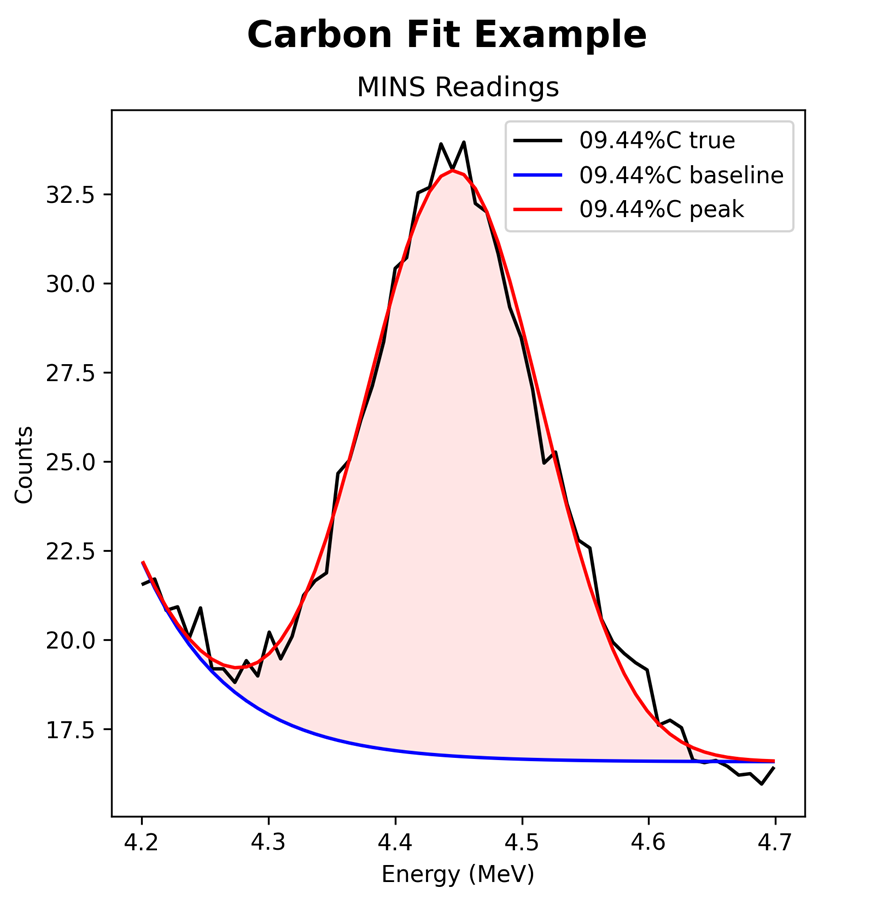
\includegraphics[width=.3\linewidth]{Figures/peakfitting.png}
    \caption{Peak Fitting Example}
    \label{fig:peakfittingexample} 
  \end{figure}
\end{frame}

\begin{frame}
  \frametitle{Prediction}
  \begin{itemize}
    \item Peak area $\rightarrow$ carbon content
    \item Train linear regression on outer values
    \item Mean Squared Error: 7.56223e-06
  \end{itemize}
  % peakfitresults.png
  \begin{figure}
      \centering
      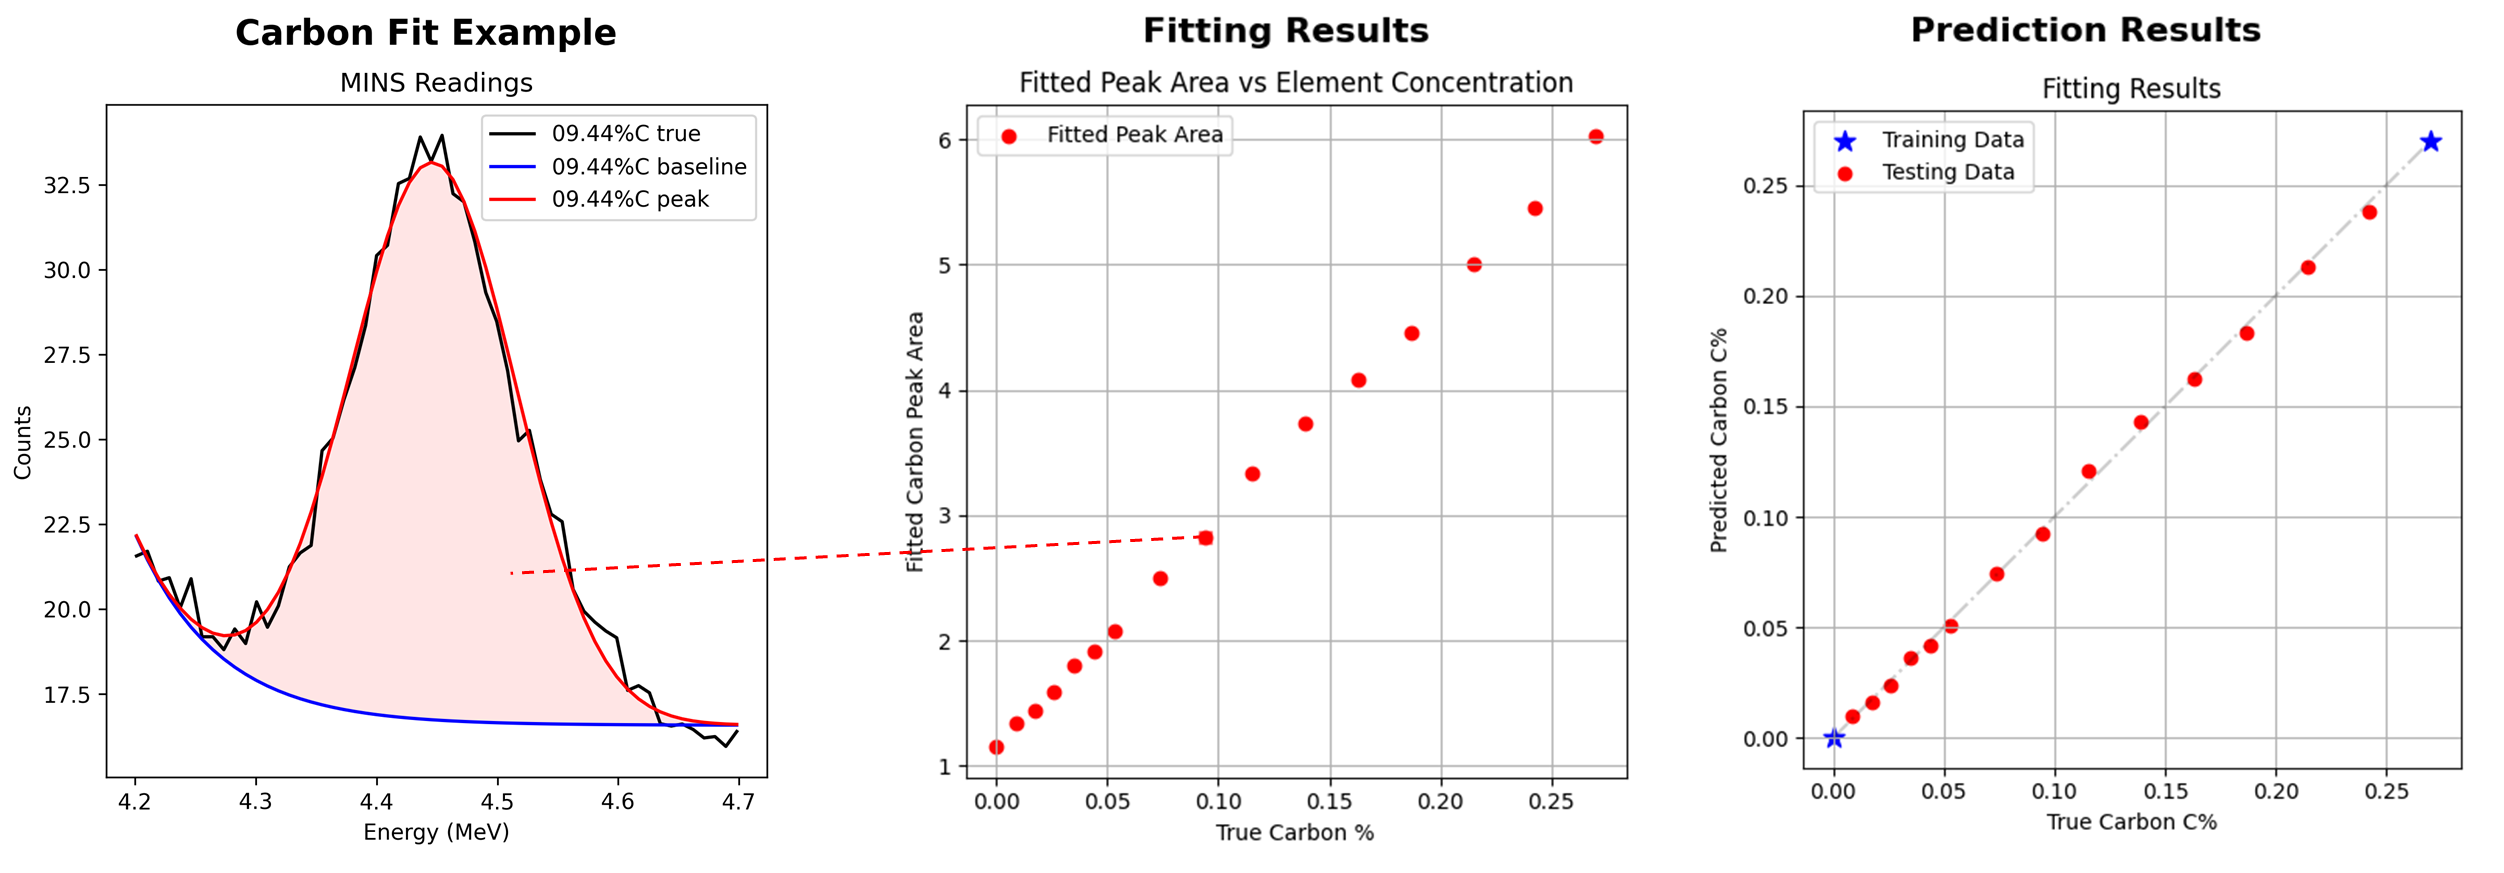
\includegraphics[width=\linewidth]{Figures/peakfitresults.png}
      \caption{Peak Fitting Results}
      \label{fig:peakfitresults}
  \end{figure}
\end{frame}

\begin{frame}
  \frametitle{Limitations}
  \begin{itemize}
    \item Requires manual element window per element
    \item Peaks may overlap $\rightarrow$ difficult for generalization
  \end{itemize}
\end{frame}

%--------- PAPER REVIEW ----------------------
\section{Paper Review}
\begin{frame}
  \frametitle{Paper Review}
  \begin{itemize}
    \item GEANT4-based study on tagged neutron method (TNM)
    \item Goal: detect explosives via C/N/O signature
  \end{itemize}
  % paperreview.png
  \begin{figure}
      \centering
      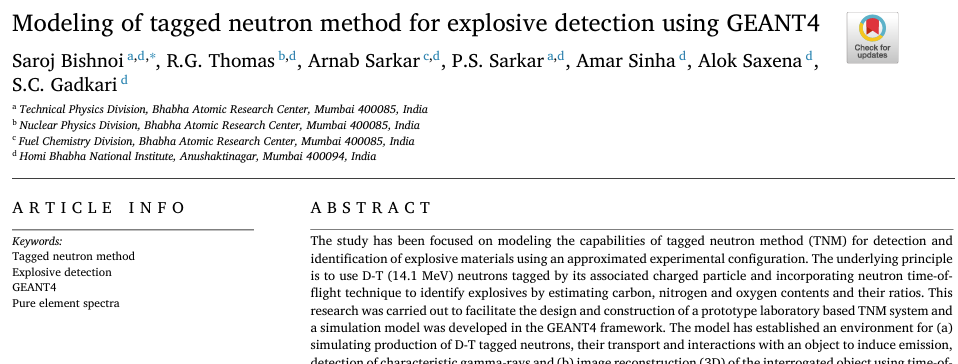
\includegraphics[width=\linewidth]{Figures/paperreview.png}
      \caption{Paper Review}
      \label{fig:paperreview}
  \end{figure}
\end{frame}

\begin{frame}
  \frametitle{Tagged Neutron Method}
  \begin{itemize}
    \item Uses alpha-neutron coincidence
    \item Measures within a known cone of interaction
  \end{itemize}
  %  Schematicrepresentationofassociatedparticlebasedtaggedneutronmethod.png
  \begin{figure}
      \centering
      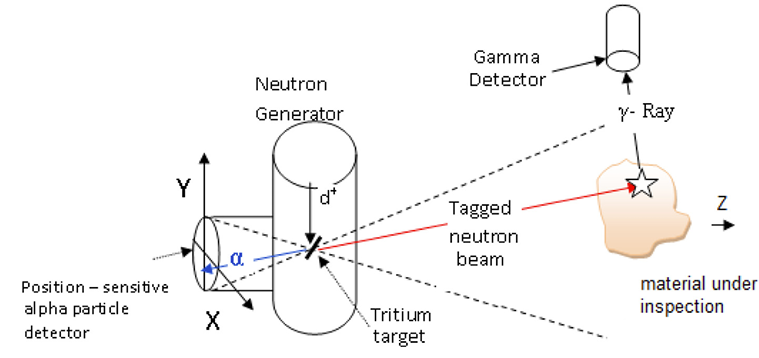
\includegraphics[width=.5\linewidth]{Figures/Schematicrepresentationofassociatedparticlebasedtaggedneutronmethod.png}
      \caption{Schematic of Tagged Neutron Method}
      \label{fig:taggedneutronmethod}
  \end{figure}
\end{frame}

\begin{frame}
  \frametitle{Component Fitting - Training}
  \begin{itemize}
    \item Generate pure-element spectra
    \item Use as reference basis for decomposition
  \end{itemize}
  % simulatedspectra.png
  \begin{figure}
      \centering
      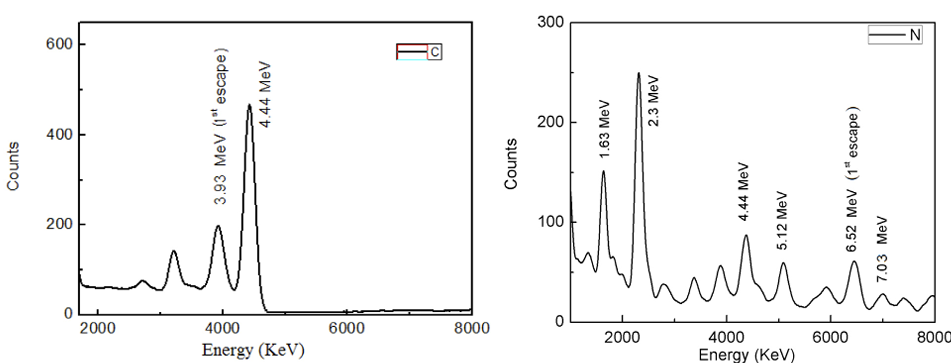
\includegraphics[width=.5\linewidth]{Figures/simulatedspectra.png}
      \caption{Simulated Spectra}
      \label{fig:simulatedspectra}
  \end{figure}

\end{frame}

\begin{frame}
  \frametitle{Component Fitting - Testing}
  \begin{itemize}
    \item Fit unknown spectrum as weighted sum
    \item Coefficients = estimated element ratios
    \item Fit optimized with L-M algorithm
  \end{itemize}
  % block for fitting function
  \begin{block}{Fitting Function}
    \begin{equation}
      f_{fit}(x) = \sum_{i=1}^{n} w_i f_i(x)
    \end{equation}
    $$
      \text{where } w_i = \text{weight of element i}
    $$
    $$
      \text{and } f_i(x) = \text{pure element spectrum}
    $$
  \end{block}
\end{frame}

\begin{frame}
  \frametitle{Paper Results}
  \begin{itemize}
    \item \~6\% error in elemental estimates
    \item Effective for simulated detection of explosives
  \end{itemize}
  \begin{figure}
      \centering
      \begin{minipage}[b]{0.45\linewidth}
          \centering
          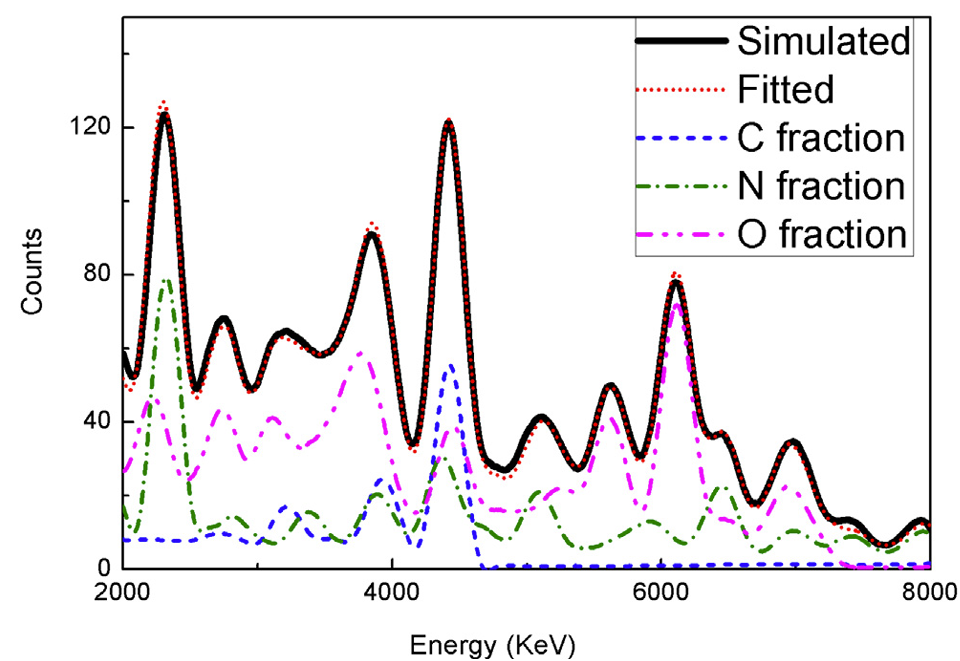
\includegraphics[width=\linewidth]{Figures/simulatedspectraanditscomponents.png}
          \caption{Simulated Spectra and Components}
          \label{fig:simulatedspectraanditscomponents}
      \end{minipage}
      \hfill
      \begin{minipage}[b]{0.45\linewidth}
          \centering
          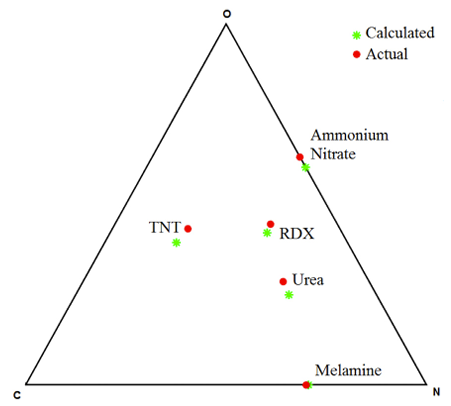
\includegraphics[width=\linewidth]{Figures/tnmresults.png}
          \caption{TNM Results}
          \label{fig:tnmresults}
      \end{minipage}
  \end{figure}
\end{frame}

%--------- APPLICATION ----------------------
\section{Application of Paper Method}
\begin{frame}
  \frametitle{Applying to MINS Data}
  \begin{itemize}
    \item Simulated spectra: C, Si, Al$_2$O$_3$, C/Si mix
    \item Initial weights: 1/n for each element
  \end{itemize}
  % DetectorSpectrumsCF.png
  \begin{figure}
      \centering
      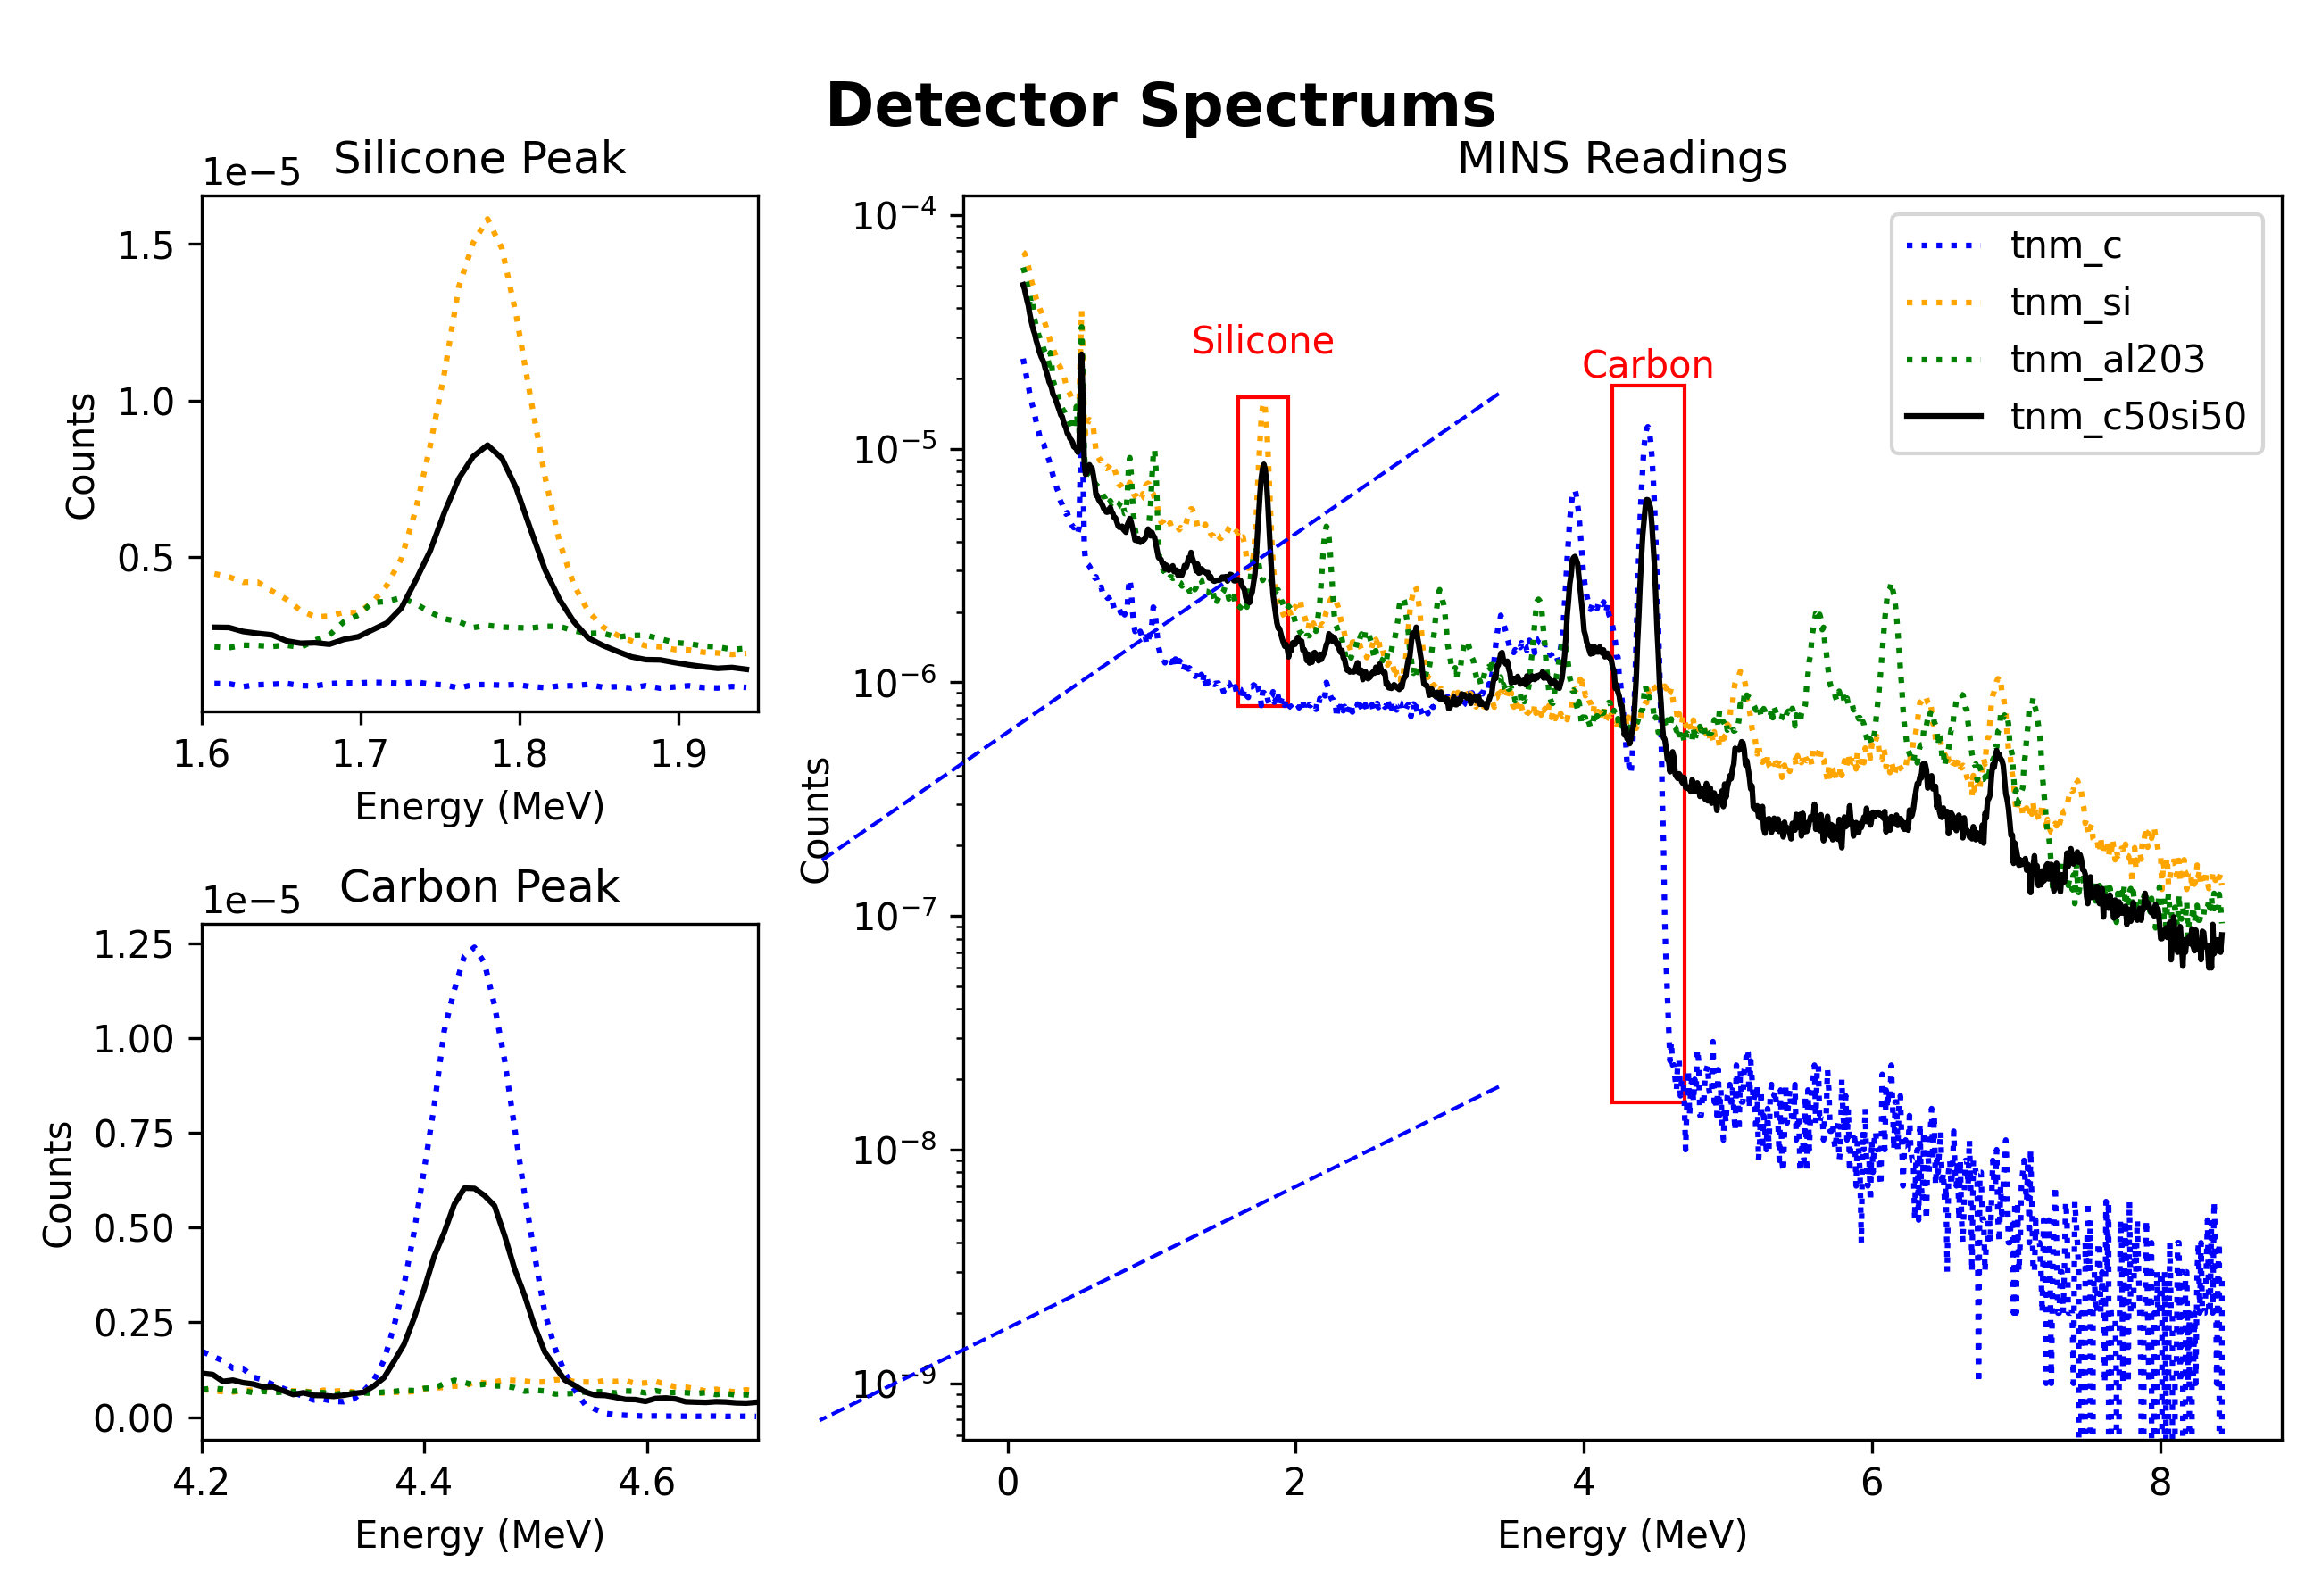
\includegraphics[width=.5\linewidth]{Figures/DetectorSpectrumsCF.png}
      \caption{Detector Spectrums}
      \label{fig:DetectorSpectrumsCF}
  \end{figure}
\end{frame}

\begin{frame}
  \frametitle{Single Result}
  \begin{itemize}
    \item Fit: C + Si = C/Si mix
    \item $0.4392 * $C + $0.5415 *$ Si = C/Si mix
  \end{itemize}
  % LinearCombinationTNMCF.png
  \begin{figure}
      \centering
      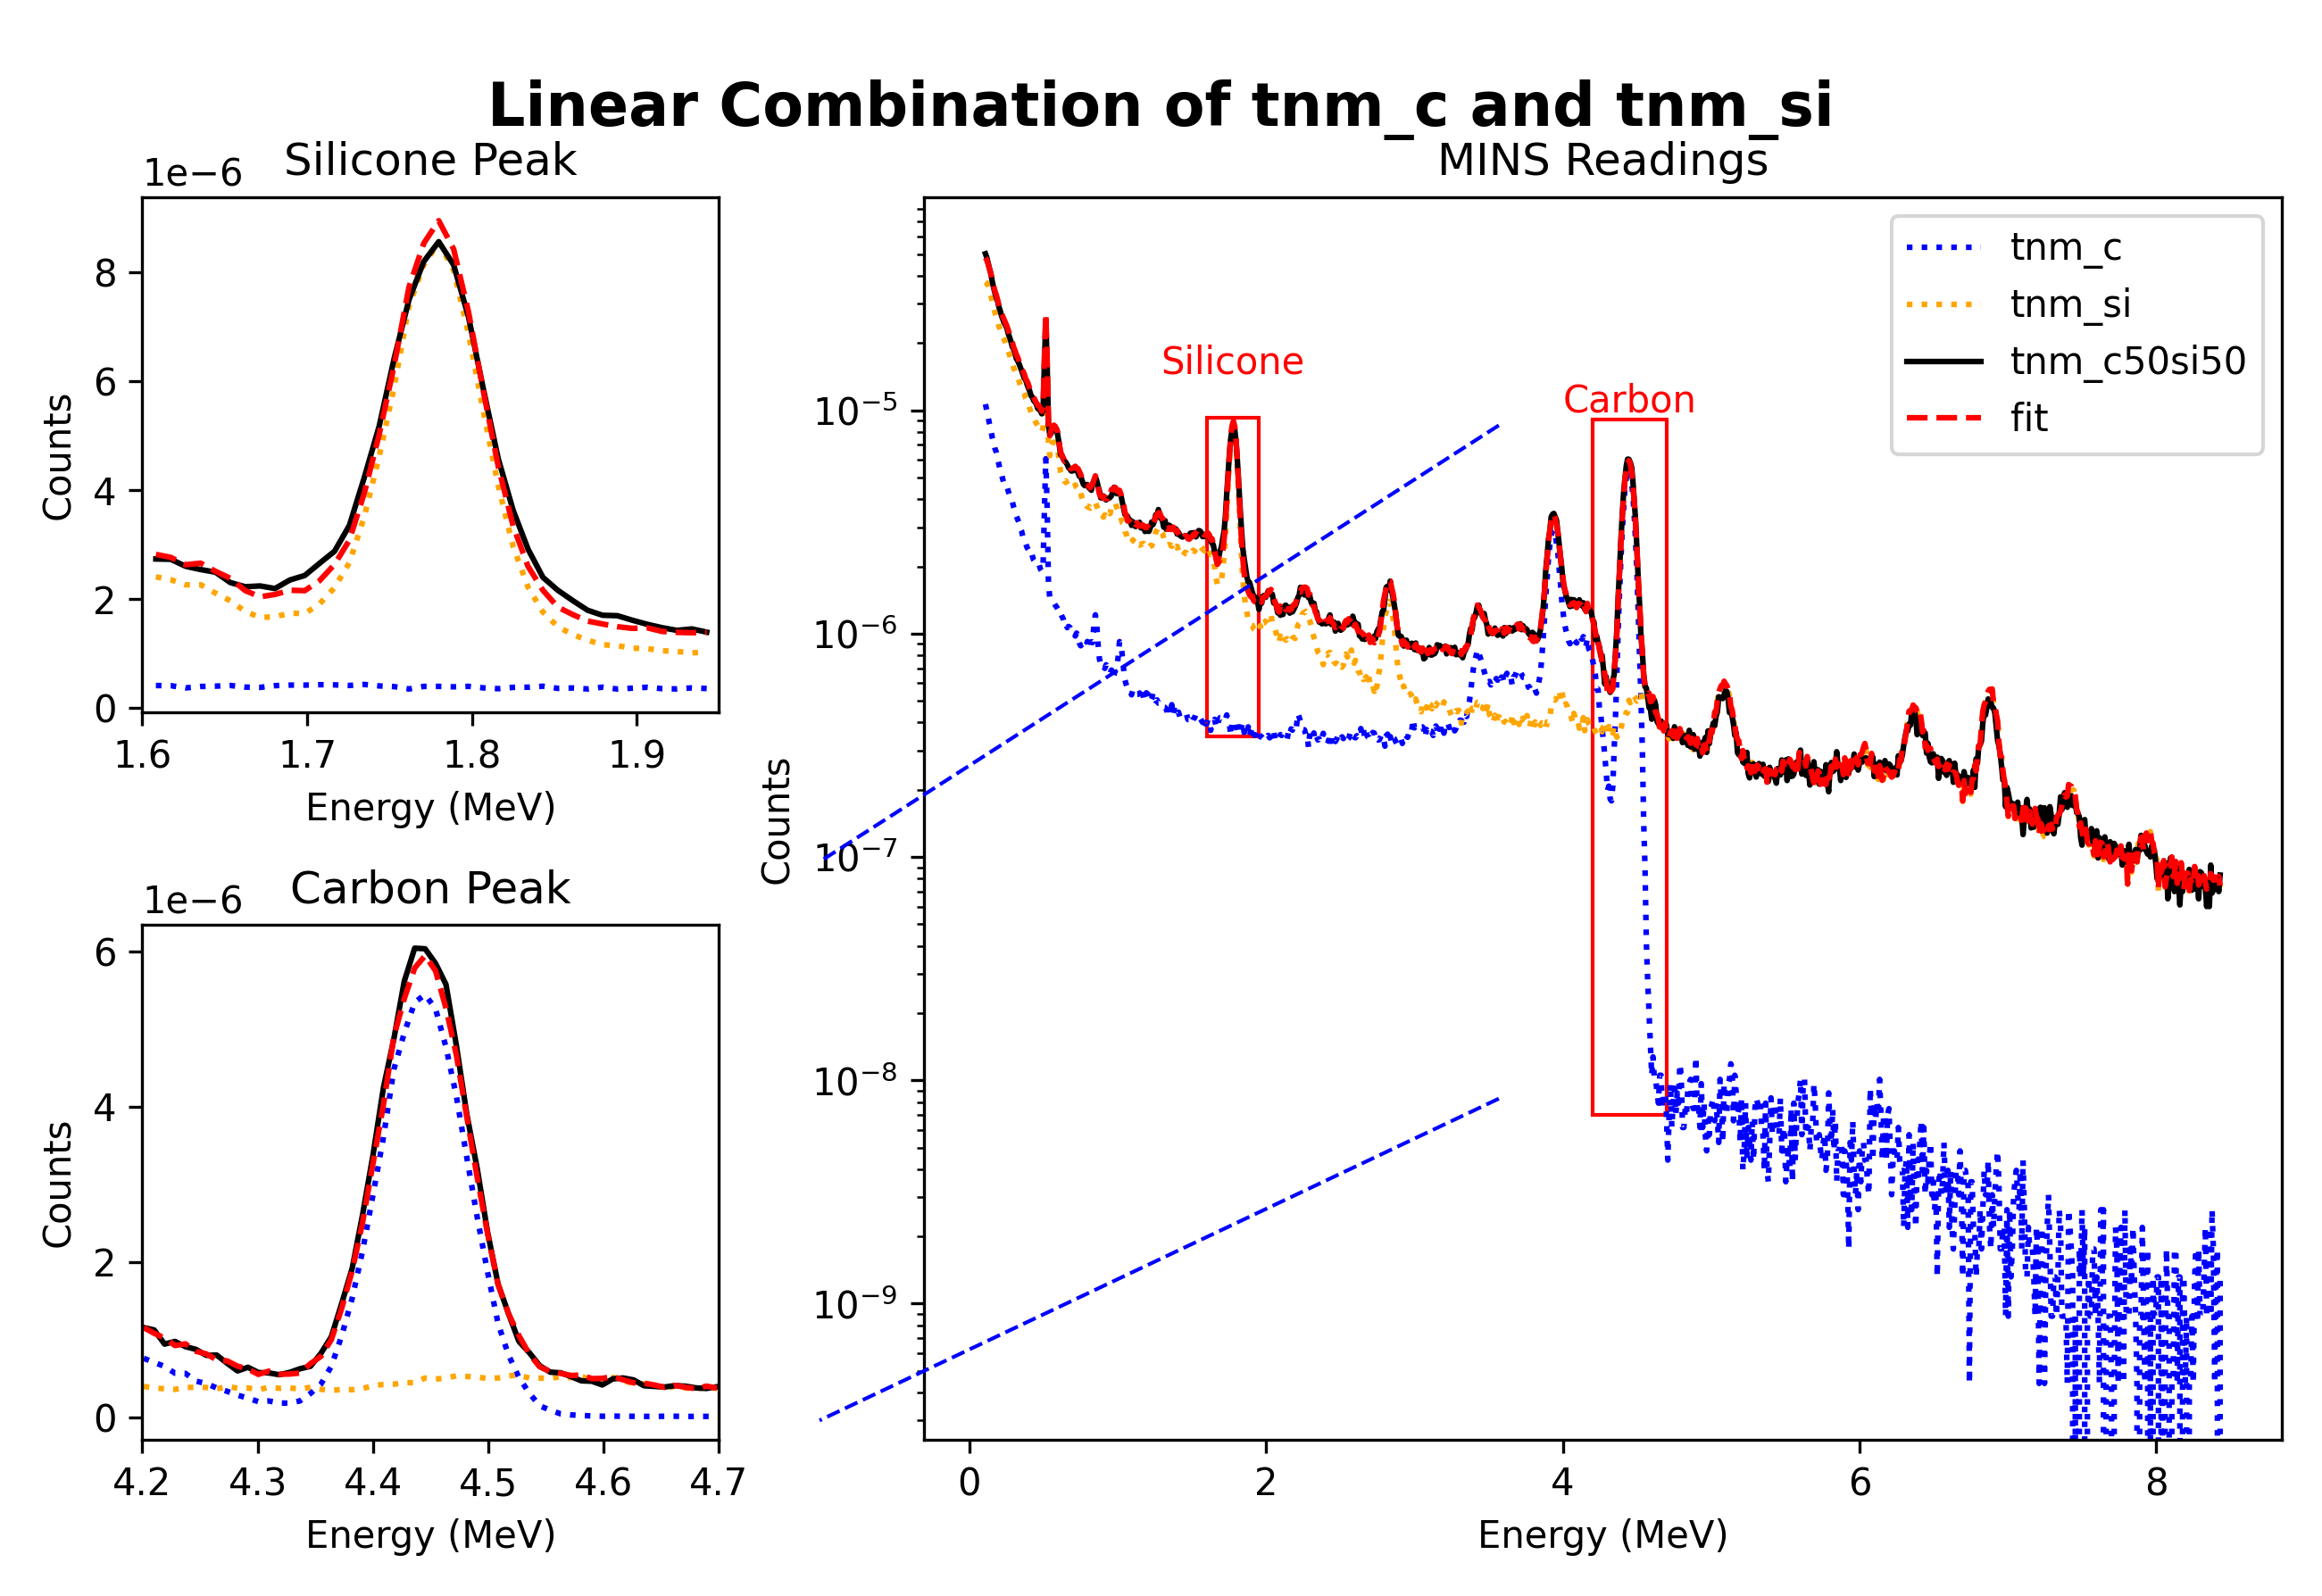
\includegraphics[width=.5\linewidth]{Figures/LinearCombinationTNMCF.png}
      \caption{Linear Combination of TNM C and Si}
      \label{fig:LinearCombinationTNMCF}
  \end{figure}
\end{frame}

\begin{frame}
  \frametitle{Ghost Element Issue}
  \begin{itemize}
     \item Including Al$_2$O$_3$ falsely contributes \~ 14\%
     \item Caution when selecting training data
     \item $0.3821 *$ C$ + 0.4448 * $Si$ + 0.1434 * $Al$_2$O$_3$ = C/Si mix
  \end{itemize}
  % LinearCombination2TNMCF.png
  \begin{figure}
      \centering
      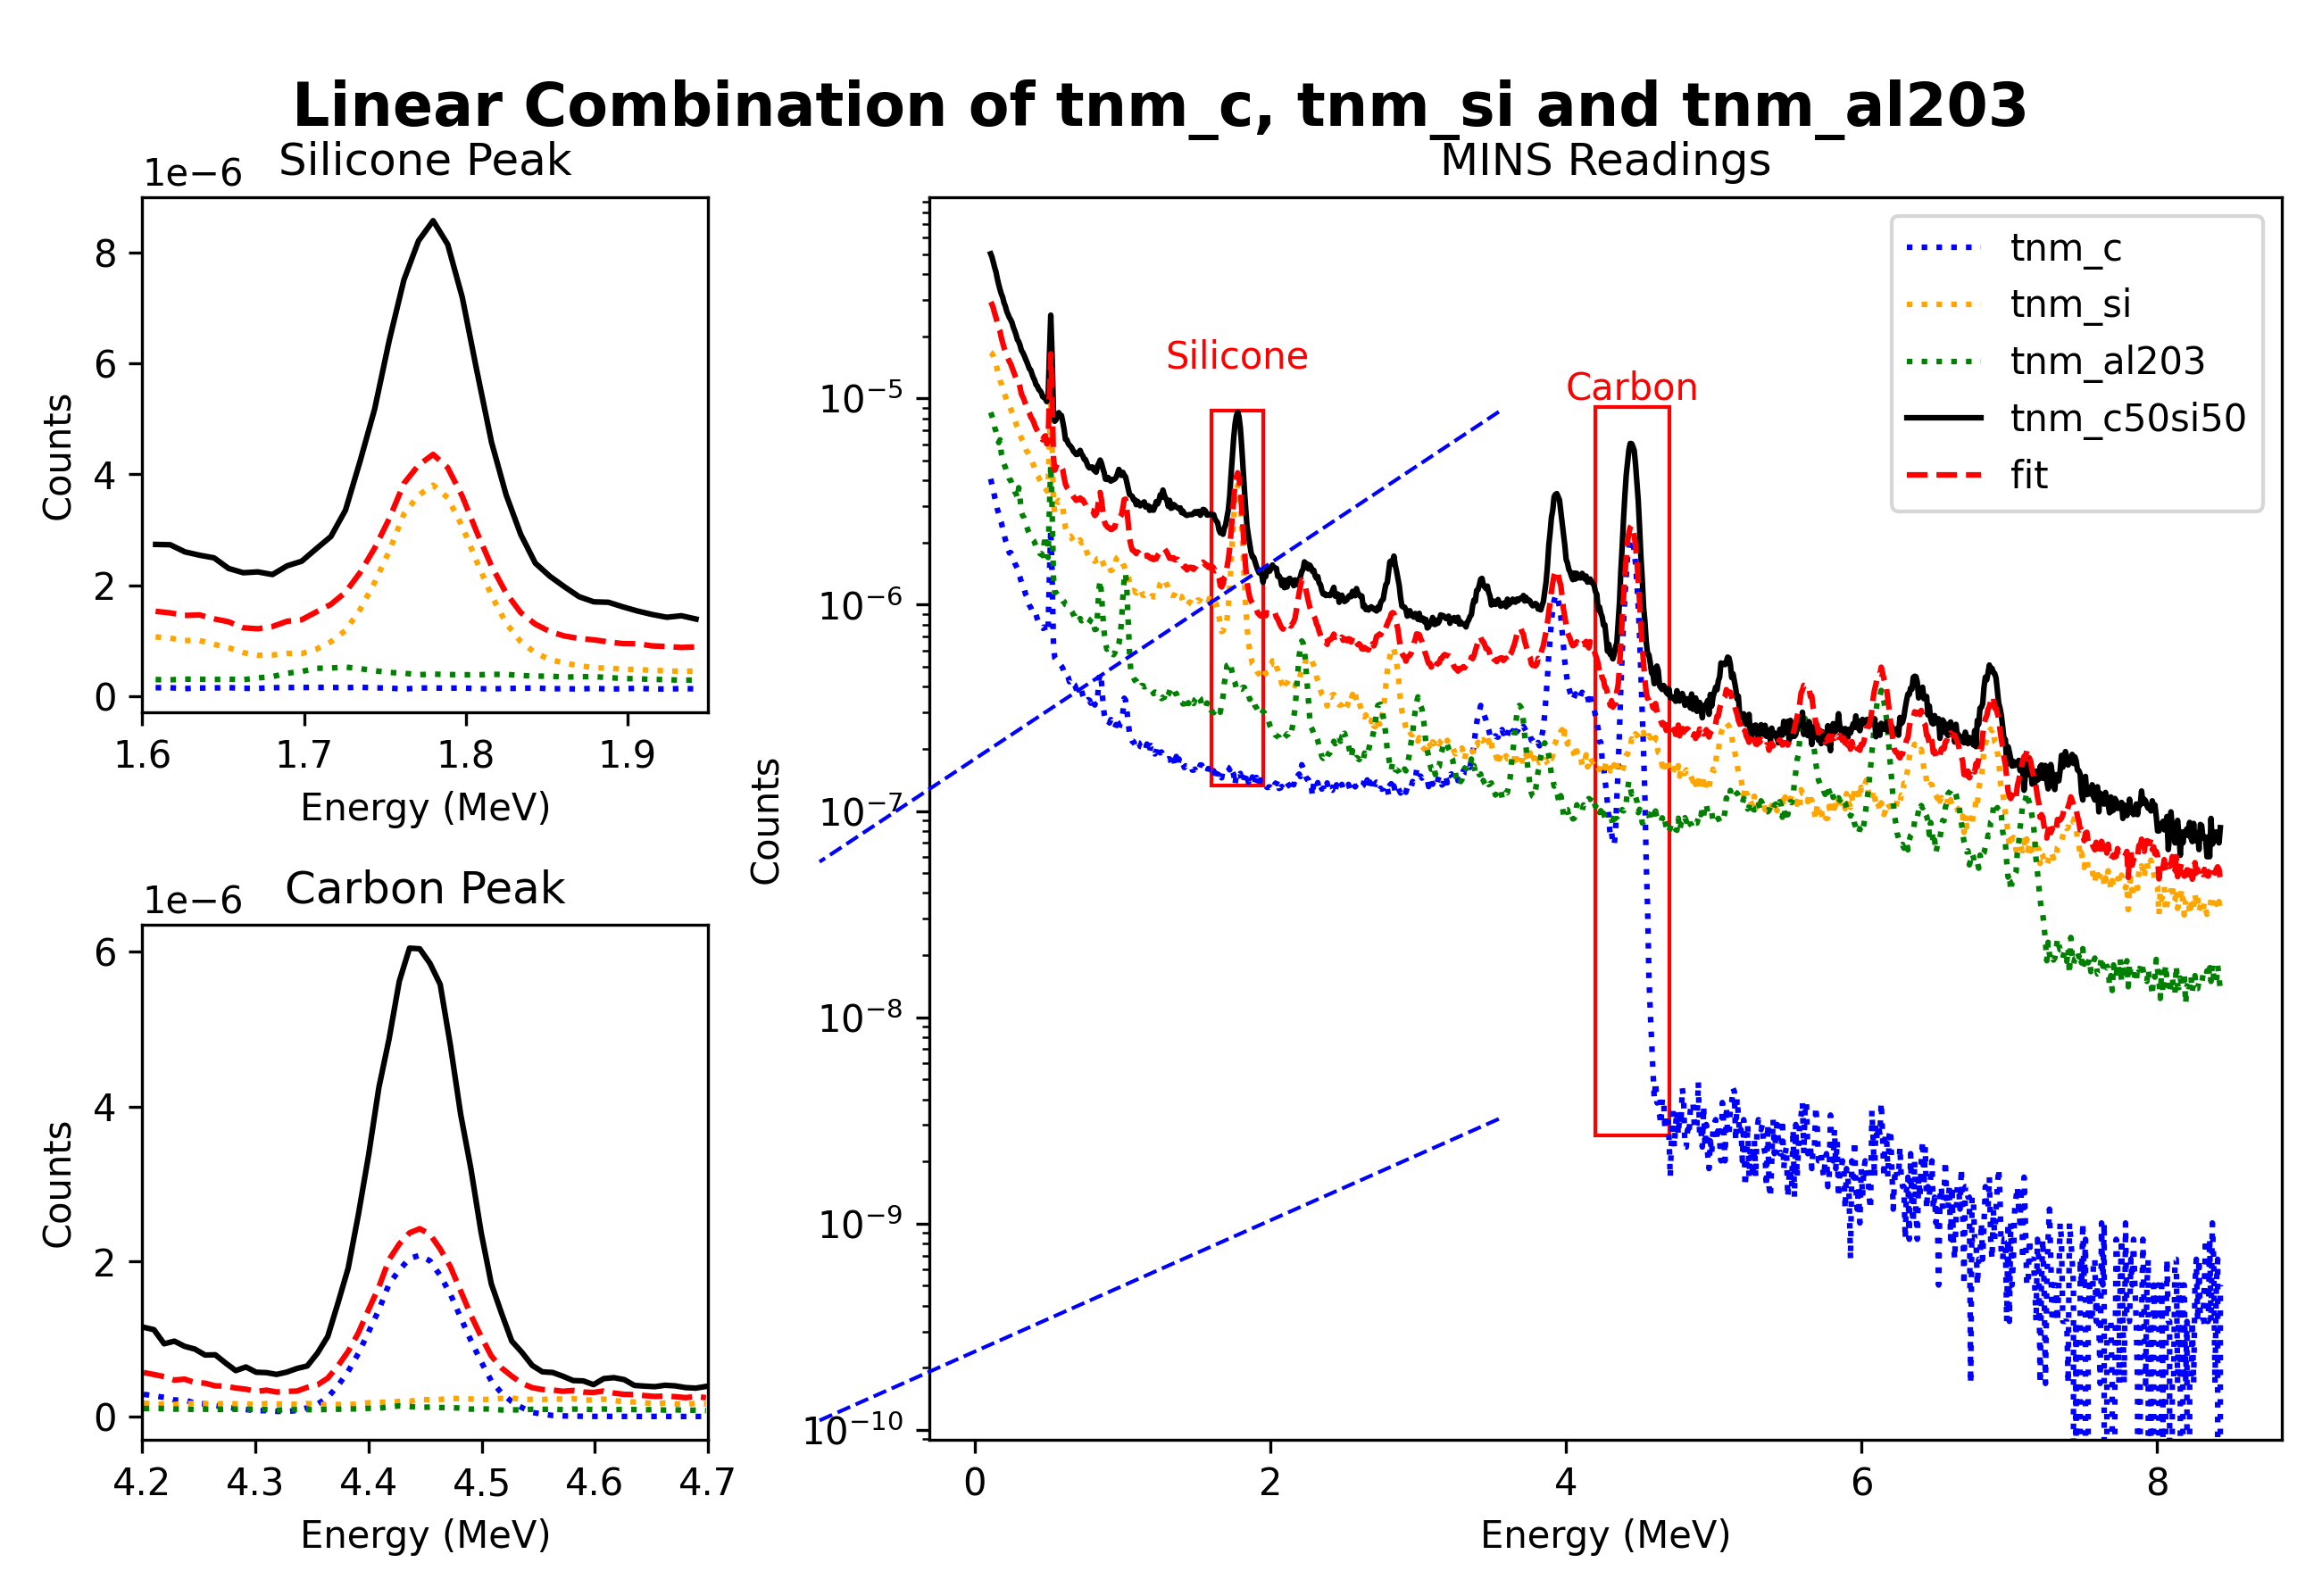
\includegraphics[width=.5\linewidth]{Figures/LinearCombination2TNMCF.png}
      \caption{Linear Combination of TNM C and Si with Al$_2$O$_3$}
      \label{fig:LinearCombination2TNMCF}
  \end{figure}
\end{frame}

\begin{frame}
  \frametitle{Limiting to Windows}
  \begin{itemize}
     \item using windows gives better Results
    %  0.44660374647308815 * C + 0.5063463294559758 * Si + 0.10138013143045811 * Al2O3 = C/Si mix
    \item $0.4466 *$ C$ + 0.5063 * $Si$ + 0.1014 * $Al$_2$O$_3$ = C/Si mix
  \end{itemize}
  % LinearCombination2TNMCF.png
  \begin{figure}
      \centering
      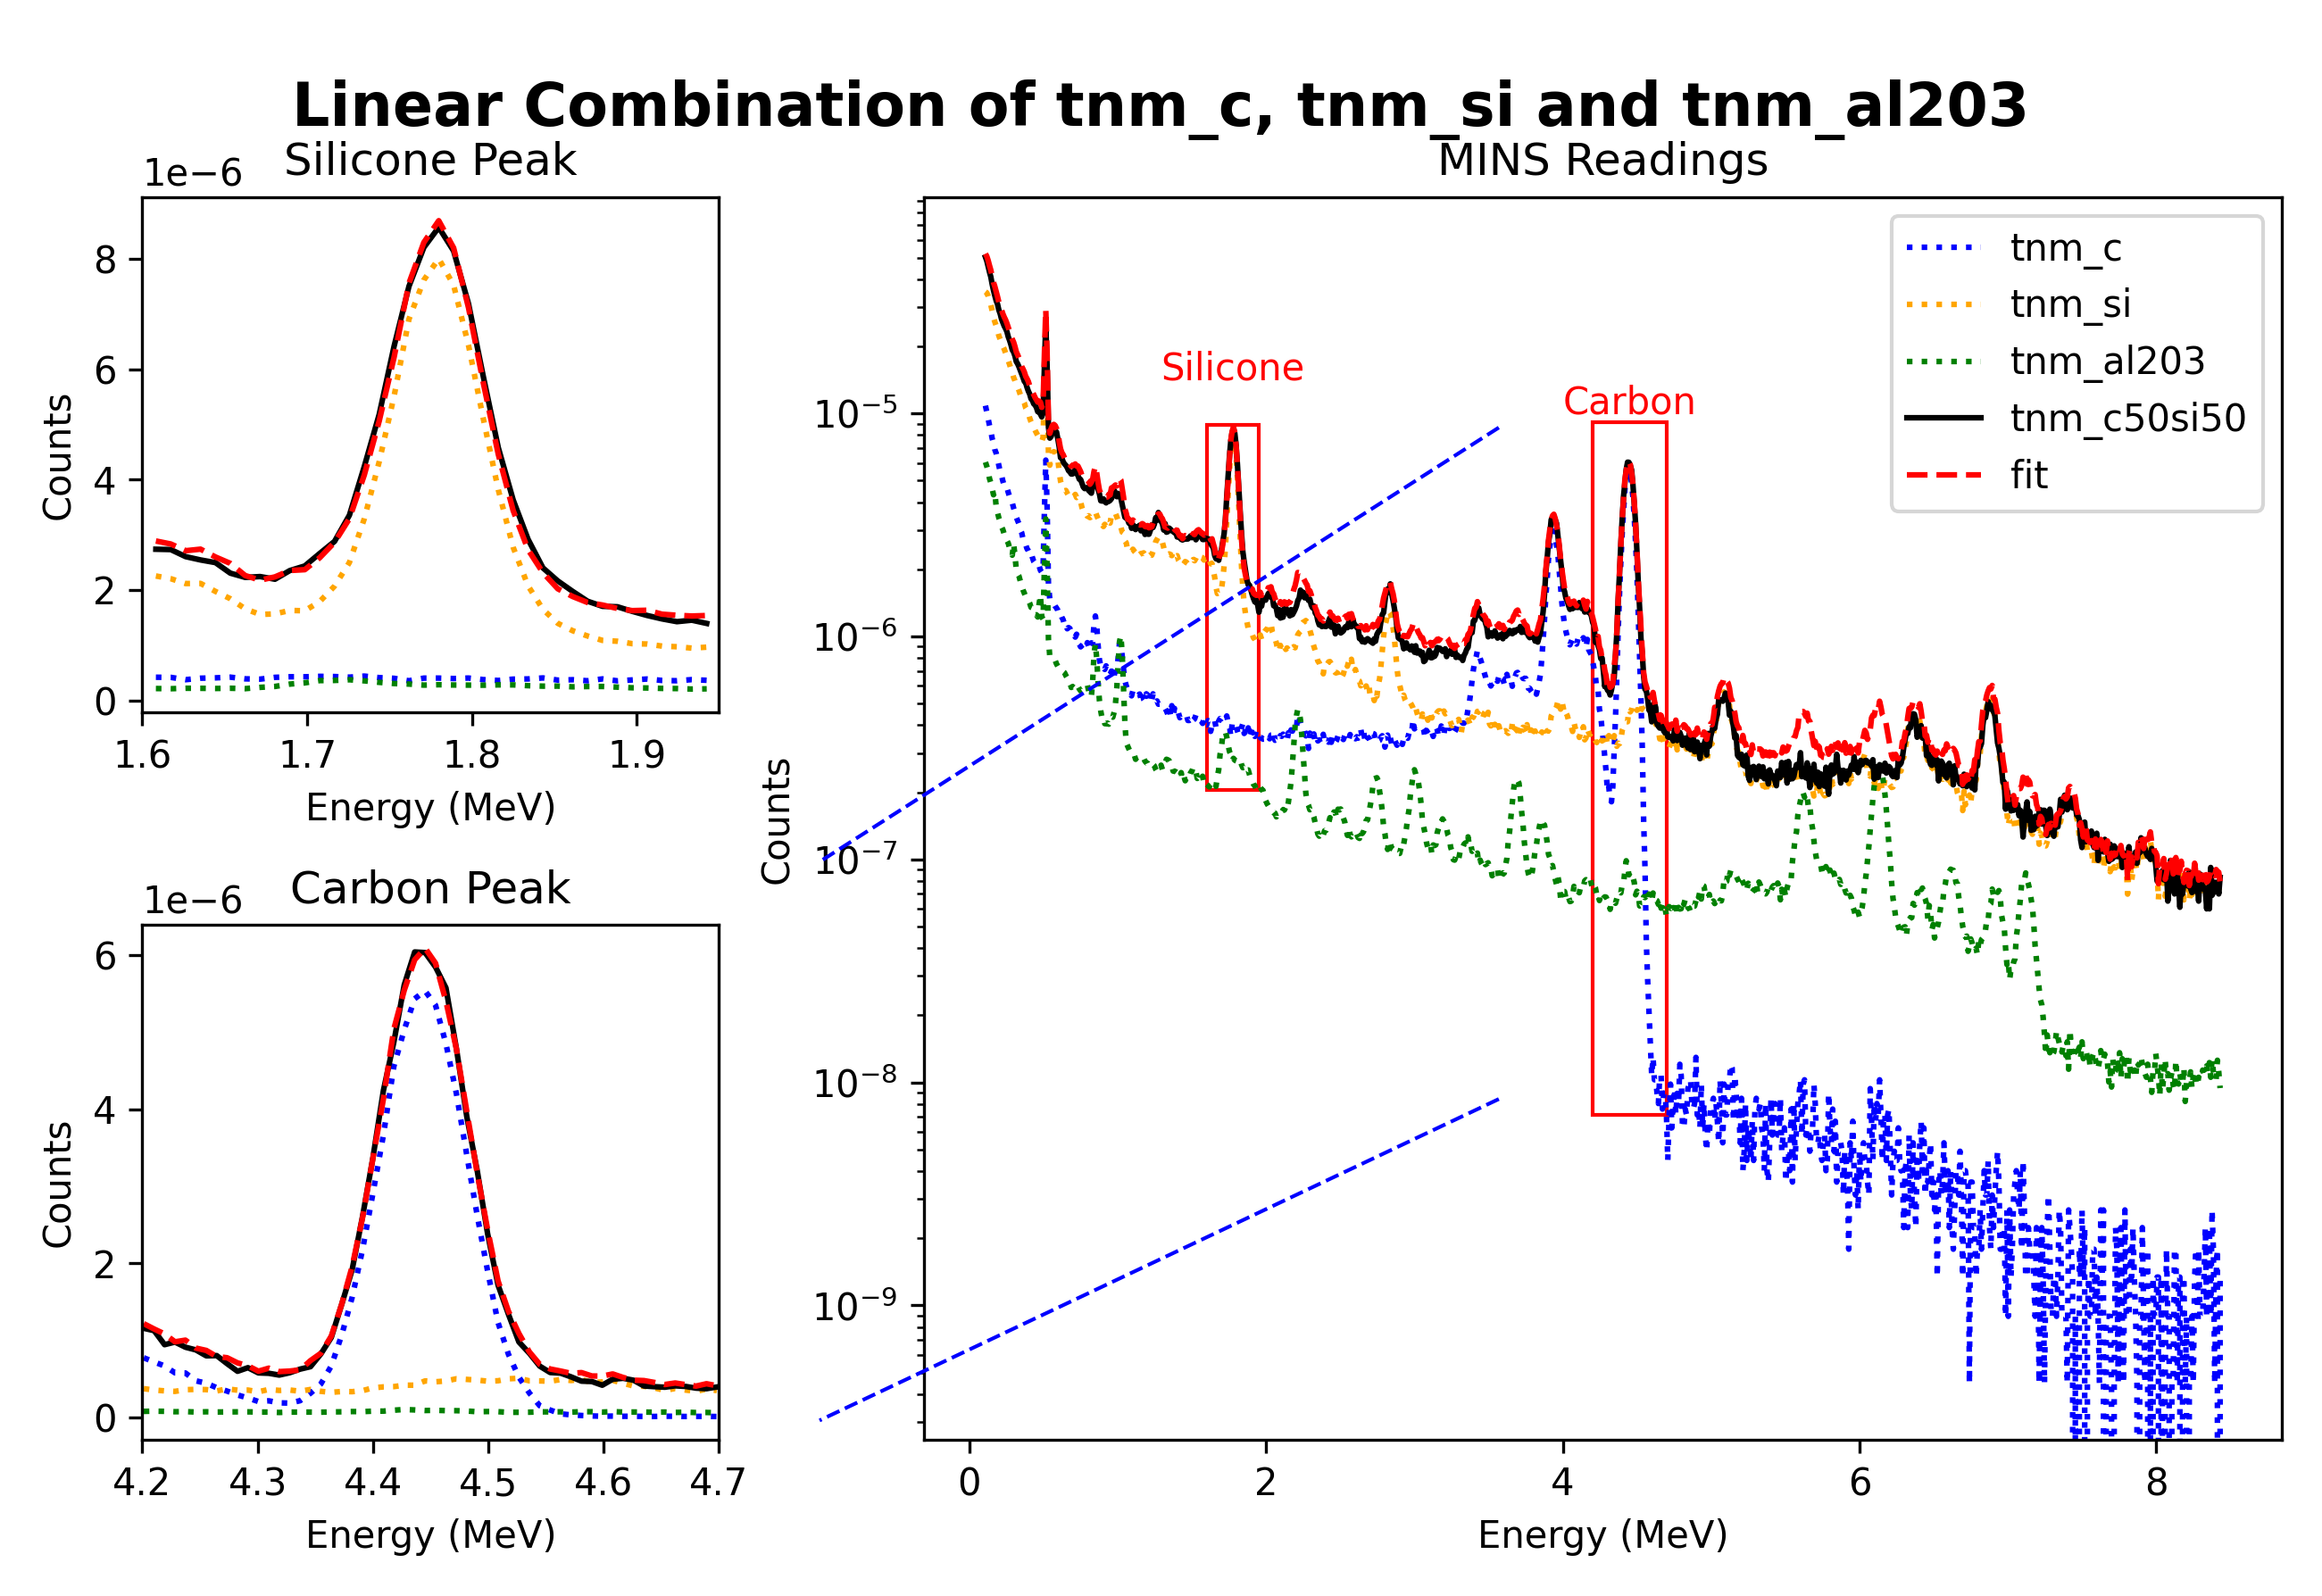
\includegraphics[width=.5\linewidth]{Figures/LinearCombination3TNMCF.png}
      \caption{Linear Combination of TNM C and Si with Al$_2$O$_3$ using Windows}
      \label{fig:LinearCombination3TNMCF}
  \end{figure}
\end{frame}

\begin{frame}
  \frametitle{Results}
  \begin{itemize}
    \item Balances peak accuracy with generalization
    \item Promising method for element quantification
  \end{itemize}
  % componentfitting.png
  \begin{figure}
      \centering
      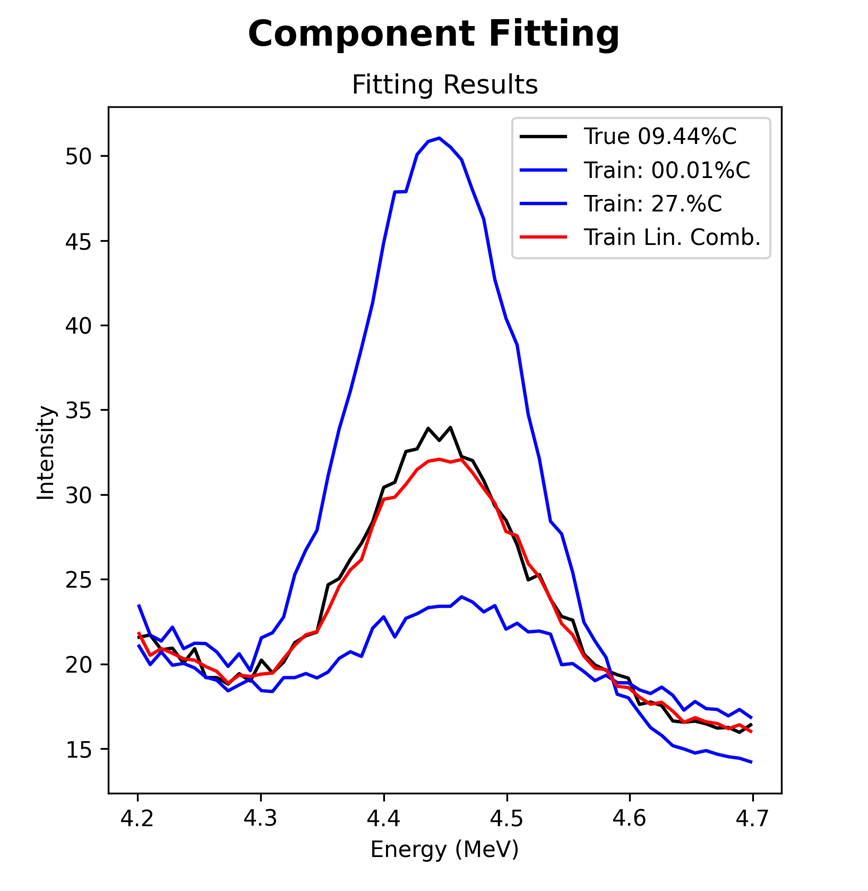
\includegraphics[width=.5\linewidth]{Figures/componentfitting.png}
      \caption{Component Fitting Results}
      \label{fig:componentfitting}
  \end{figure}
\end{frame}

\begin{frame}
  \frametitle{Full Results}
  \begin{figure}
      \centering
      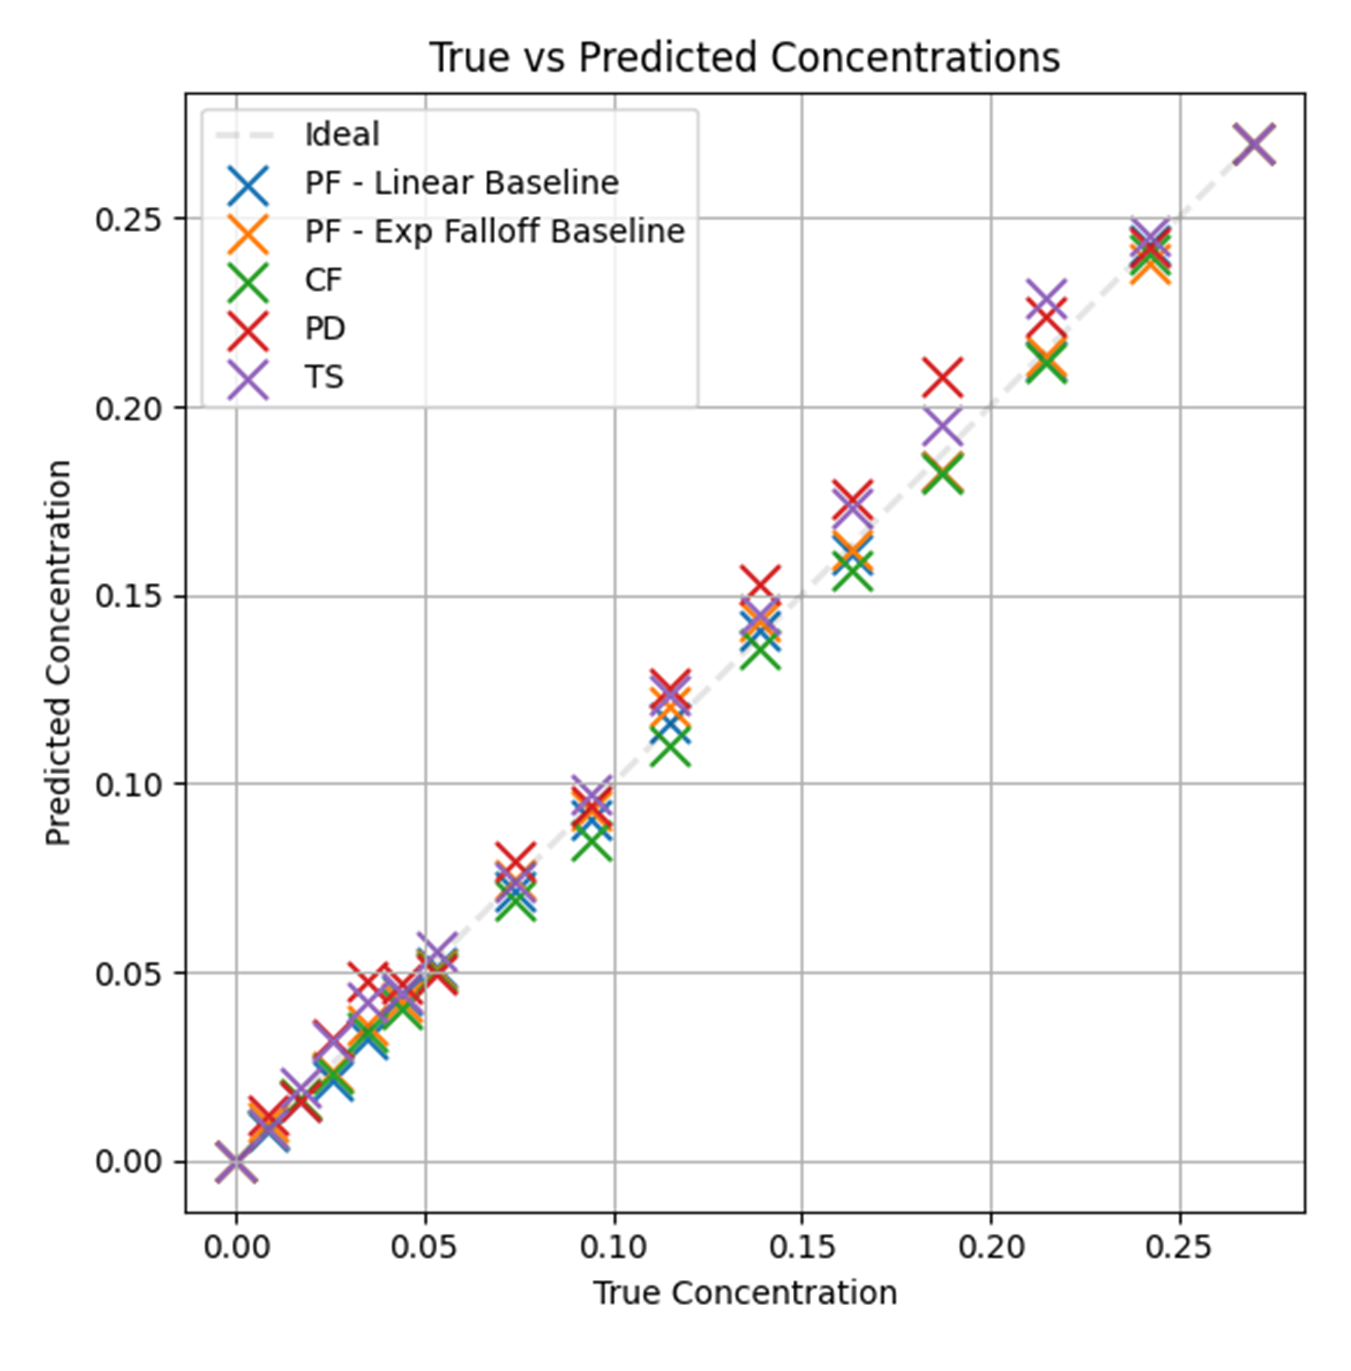
\includegraphics[width=.5\linewidth]{Figures/fullresults.png}
      \caption{Full Results}
      \label{fig:fullresults}
  \end{figure}
\end{frame}

\begin{frame}
  \frametitle{MAE comparison}
  \begin{table}[h!]
    \centering
    \begin{tabular}{|l|r|}
    \hline
    \textbf{Spectrum Analysis Method} & \textbf{MSE} \\
    \hline
    Peak Fitting Linear Baseline     & \(6.00647 \times 10^{-6}\) \\
    Peak Fitting Exponential Baseline & \(7.56223 \times 10^{-6}\) \\
    Component Fitting                  & \(1.89773 \times 10^{-5}\) \\
    Perpendicular Drop                 & 0.00741817 \\
    Tangent Skim                       & 0.00504626 \\
    \hline
    \end{tabular}
    \caption{Mean Squared Error (MSE) by Spectrum Analysis Method}
    \label{tab:spectrum-analysis} 
  \end{table}
\end{frame}


\begin{frame}
  \frametitle{Conclusion}
  \begin{itemize}
    % transcript: *In summary, I explored a paper on spectral deconvolution and applied the curve-fitting method on the projects data. I compared this to the other methods. This method shows promise for real-time field analysis, offering a flexible alternative to peak-based approaches.*
    \item Explored spectral deconvolution paper
    \item Applied curve-fitting method to project data
    \item Compared with other methods
    \item Promising for real-time field analysis
    \item Flexible alternative to peak-based approaches
  \end{itemize}
\end{frame}

\begin{frame}
  \frametitle{Future Work}
  % *The simulations take a long time to run, about 5 days for 10 to the power of 9 histories. although access to the atlas hpc is available to run around 20 jobs at once, this is still a long time to wait for results, especially when testing thousands of samples as you would in a field. I will be looking into the accuracy of reversing the deconvolution method. By reversing the process, I can generate a spectrum from a known mixture of elements. This will allow me to test the accuracy of the deconvolution methods without having to wait for the long simulation times.*
  \begin{itemize}
    \item Simulations take long time (5 days for 10\textsuperscript{9} histories)
    \item Atlas HPC: run 20 jobs at once, still long wait
    \item Future: reverse deconvolution method
    \item Generate spectrum from known mixture
    \item Test accuracy of deconvolution methods
  \end{itemize}
\end{frame}

\begin{frame}
  \frametitle{Acknowledgments}
  \begin{itemize}
    \item USDA for internship opportunity
    \item Dr. Andrzej Korzeniowski for guidance
    \item Dr. Galina Yakubova, Dr. Aleksandr Kavetskiy, Dr. Allen Tobert for collaboration
    \item Atlas HPC for computational resources
  \end{itemize}
\end{frame}



%----------- REFERENCES  -------------
%----------- No editing in references section ----------
%----------- edit only in References.bib ----------
\section{Bibliography}
\begin{frame}[allowframebreaks]
  \begin{thebibliography}{11}

    \bibitem{copley2013}
    J. Copley, ``Introduction to Neutron Scattering,'' presented at the Summer School on the Fundamentals of Neutron Scattering, NIST Center for Neutron Research, Jul. 17, 2013. [Online]. Available: \url{https://www.ncnr.nist.gov/summerschool/ss13/pdf/SS2013_Lecture_Copley.pdf}
    
    \bibitem{werner2017}
    C. J. Werner \textit{et al.}, \textit{MCNP User's Manual Code Version 6.2}. Los Alamos National Laboratory Tech. Rep. LA-UR-17-29981, Los Alamos, NM, USA, Oct. 2017.
    
    \bibitem{kavetskiy2024}
    A. G. Kavetskiy, G. N. Yakubova, S. A. Prior, and H. A. Torbert III, ``Monte-Carlo simulations for soil content determinations on Atlas,'' \textit{SCINet Newsletter}, 2024. [Online]. Available: \url{https://scinet.usda.gov/news/newsletter}
    
    \bibitem{bates2022}
    C. R. Bates, S. R. Bolding, C. J. Josey, J. A. Kulesza, C. J. Solomon Jr., and A. J. Zukaitis, ``The MCNPTools Package: Installation and Use,'' Los Alamos National Laboratory Tech. Rep. LA-UR-22-28935, Los Alamos, NM, USA, Aug. 2022, doi: \url{10.2172/1884737}.
    
    \bibitem{virtanen2020}
    P. Virtanen \textit{et al.}, ``SciPy 1.0: Fundamental Algorithms for Scientific Computing in Python,'' \textit{Nature Methods}, vol. 17, no. 3, pp. 261--272, 2020.
    
    \bibitem{usdaimage}
    ``d2399-1'' by USDAgov is licensed under CC BY 2.0.
    
    \bibitem{gehl2007}
    R. J. Gehl and C. W. Rice, ``Emerging technologies for in situ measurement of soil carbon,'' \textit{Climatic Change}, vol. 80, pp. 43--54, 2007, doi: \url{https://doi.org/10.1007/s10584-006-9150-2}.
    
    \bibitem{wielopolski2011}
    L. Wielopolski, A. Chatterjee, S. Mitra, and R. Lal, ``In situ determination of Soil carbon pool by inelastic neutron scattering: Comparison with dry combustion,'' \textit{Geoderma}, vol. 160, no. 3, pp. 394--399, 2011, doi: \url{https://doi.org/10.1016/j.geoderma.2010.10.009}.
    
    \bibitem{matejovic1997}
    I. Matejovic, ``Determination of carbon and nitrogen in samples of various soils by the dry combustion,'' \textit{Communications in Soil Science and Plant Analysis}, vol. 28, no. 17--18, pp. 1499--1511, 1997.
    
    \bibitem{ohaver2025}
    T. O'Haver, \textit{A pragmatic introduction to signal processing: with applications in scientific measurement}, University of Maryland, Feb. 2025. [Online]. Available: \url{https://terpconnect.umd.edu/~toh/spectrum/TOC.html}
    
    \bibitem{bishnoi2019}
    S. Bishnoi, R. G. Thomas, A. Sarkar, P. S. Sarkar, A. Sinha, A. Saxena, and S. C. Gadkari, ``Modeling of tagged neutron method for explosive detection using GEANT4,'' \textit{Nuclear Instruments and Methods in Physics Research Section A}, vol. 923, pp. 26--33, 2019.
    
    \end{thebibliography}
\end{frame}
\end{document}